\section{Supplemental Tables and Figures}
\setcounter{table}{0}
\setcounter{figure}{0}
\renewcommand{\thetable}{S\arabic{table}}
\renewcommand{\thefigure}{S\arabic{figure}}
\setcounter{page}{1}

\begin{table*}[h]
\renewcommand{\familydefault}{\sfdefault}\normalfont
\begin{tableminipage}{\textwidth}
\captionsetup{width=\textwidth}
\centering
\caption{\bf Number of differentially expressed genes and accessible chromatin regions detected between liver, lung, and kidney tissues
\label{tab:diff_gene}}
\end{tableminipage}
\begin{tableminipage}{\textwidth}
\begin{tabularx}{\textwidth}{cll|XXX}
\hline 
& & & & \center{Tissue comparison} & \\
& & & Liver vs Lung & Liver vs Kidney & Lung vs Kidney \\
\hline
%%%%%%%%%%%%%%%%
\parbox[t]{5mm}{\multirow{6}{*}{\rotatebox[origin=c]{90}{q-value < 0.1}}} & 
Genes & Up-regulated & 2,473 (20.8\footnote{Percentage of all tested genes.\label{fn:total_perc_gene}}) & 2,123 (17.9\footref{fn:total_perc_gene}) & 2,246 (18.9\footref{fn:total_perc_gene}) \\
& & Down-regulated & 3,236 (27.2\footref{fn:total_perc_gene}) & 1,441 (12.1\footref{fn:total_perc_gene}) & 2,527 (21.3\footref{fn:total_perc_gene}) \\
& & Total & 5,709 (48.0\footref{fn:total_perc_gene}) & 3,564 (30.0\footref{fn:total_perc_gene}) & 4,773 (40.2\footref{fn:total_perc_gene}) \\
\cline{2-6}
& Chromatin Regions & Increased accessibility & 20,194 (19.6\footnote{Percentage of all tested chromatin regions prior to merging adjacent genomic windows.\label{fn:total_perc_chrom}}) & 15,252 (12.9\footref{fn:total_perc_chrom}) & 19,202 (17.4\footref{fn:total_perc_chrom}) \\
& & Decreased accessibility & 20,603 (19.7\footref{fn:total_perc_chrom}) & 12,796 (11.4\footref{fn:total_perc_chrom}) & 12,967 (11.2\footref{fn:total_perc_chrom}) \\
& & Total & 40,797 (39.3\footref{fn:total_perc_chrom}) & 28,048 (24.3\footref{fn:total_perc_chrom}) & 32,169 (28.6\footref{fn:total_perc_chrom}) \\
\hline
\end{tabularx}
\end{tableminipage}
\end{table*}

\begin{table*}[h]
\renewcommand{\familydefault}{\sfdefault}\normalfont
\begin{tableminipage}{\textwidth}
\captionsetup{width=\textwidth}
\centering
\caption{\bf Number of genes with eQTL detected in liver, lung, and kidney tissues
\label{tab:eqtl_mapping}}
\end{tableminipage}
\begin{tableminipage}{\textwidth}
\begin{tabularx}{\textwidth}{ll|XXX}
\hline 
& & & \center{Tissue (\%)} & \\
Procedure & eQTL type & Liver & Lung & Kidney \\
\hline
%%%%%%%%%%%%%%%%
Method 1\footnote{Multi-stage conditional regression analysis with genome-wide FDR < 0.1. \label{fn:method_one}} & All & 520 (6.2\footnote{Percentage of all tested genes.\label{fn:total_perc}}) & 478 (4.2\footref{fn:total_perc}) & 739 (7.3\footref{fn:total_perc}) \\
& Local\footnote{10 Mb upstream or downstream of gene TSS. \label{fn:local_eqtl}} & 400 (76.9\footnote{Percentage of genes with genome-wide eQTL.\label{fn:gw_eqtl_perc}}) & 369 (77.2\footref{fn:gw_eqtl_perc}) & 601 (81.3\footref{fn:gw_eqtl_perc}) \\
& Distal\footnote{More than 10 Mb upstream or downstream of gene TSS or on another chromosome. \label{fn:distal_eqtl}} & 132 (25.4\footref{fn:gw_eqtl_perc}) & 112 (23.4\footref{fn:gw_eqtl_perc}) & 148 (20.0\footref{fn:gw_eqtl_perc}) \\
\hline
% %%%%%%%%%%%%%%%%
Method 2\footnote{Single-step regression analysis with chromosome-wide FDR < 0.1. \label{fn:method_two}} & All & 2,587 (30.8\footref{fn:total_perc}) & 2,069 (18.2\footref{fn:total_perc}) & 3,191 (31.6\footref{fn:total_perc}) \\
& Local\footref{fn:local_eqtl} & 1,749 (67.6\footnote{Percentage of genes with chromosome-wide eQTL.\label{fn:cw_eqtl_perc}}) & 1,498 (72.4\footref{fn:cw_eqtl_perc}) & 2,214 (69.4\footref{fn:cw_eqtl_perc}) \\
& Distal\footref{fn:distal_eqtl} & 838 (32.4\footref{fn:cw_eqtl_perc}) & 571 (27.6\footref{fn:cw_eqtl_perc}) & 977 (30.6\footref{fn:cw_eqtl_perc}) \\
\hline
% %%%%%%%%%%%%%%%%
Method 3\footnote{Single-step regression analysis restricted to local signals and with FWER p-value < 0.05. \label{fn:method_three}} & Local\footref{fn:local_eqtl} genome-wide & 702 (8.4\footref{fn:total_perc}) & 713 (6.3\footref{fn:total_perc}) & 955 (9.5\footref{fn:total_perc}) \\
& Local\footref{fn:local_eqtl} chromosome-wide & 1,661 (19.8\footref{fn:total_perc}) & 1,880 (16.6\footref{fn:total_perc}) & 2,102 (20.8\footref{fn:total_perc}) \\
% & chromatin mediator\footnote{Must be within 10 Mb upstream or downstream of an local-eQTL that is at least chromosome-wide significant. Additionally, chromatin mediator must possess a local c-QTL that is at least chromosome-wide significant.} & genome-wide & 38 (2.2\footnote{Percentage of genes with a chromatin mediator that have at least a chromosome-wide significant local-eQTL from local analysis.\label{fn:mediator_perc}}) & 13 (0.9\footref{fn:mediator_perc}) & 19 (1.0\footref{fn:mediator_perc}) \\
% & chromosome-wide & 99 (5.9\footref{fn:mediator_perc}) & 30 (2.0\footref{fn:mediator_perc}) & 49 (2.6\footref{fn:mediator_perc}) \\
\hline
\end{tabularx}
\end{tableminipage}
\end{table*}

\begin{table*}[h]
\renewcommand{\familydefault}{\sfdefault}\normalfont
\begin{tableminipage}{\textwidth}
\captionsetup{width=\textwidth}
\centering
\caption{\bf Number of genes with eQTL detected in liver, lung, and kidney tissues at FDR < 0.2
\label{tab:eqtl_mapping_lenient}}
\end{tableminipage}
\begin{tableminipage}{\textwidth}
\begin{tabularx}{\textwidth}{ll|XXX}
\hline 
& & & \center{Tissue (\%)} & \\
Procedure & eQTL type & Liver & Lung & Kidney \\
\hline
%%%%%%%%%%%%%%%%
Method 1\footnote{Multi-stage conditional regression analysis with genome-wide FDR < 0.2.} & All & 881 (10.5\footref{fn:total_perc}) & 811 (7.1\footref{fn:total_perc}) & 1,189 (11.8\footref{fn:total_perc}) \\
& Local\footnote{10 Mb upstream or downstream of gene TSS. \label{fn:local_eqtl}} & 568 (64.5\footref{fn:gw_eqtl_perc}) & 522 (64.4\footref{fn:gw_eqtl_perc}) & 809 (68.0\footref{fn:gw_eqtl_perc}) \\
& Distal\footnote{More than 10 Mb upstream or downstream of gene TSS or on another chromosome. \label{fn:distal_eqtl}} & 339 (38.5\footref{fn:gw_eqtl_perc}) & 301 (37.1\footref{fn:gw_eqtl_perc}) & 411 (34.6\footref{fn:gw_eqtl_perc}) \\
\hline
% %%%%%%%%%%%%%%%%
Method 2\footnote{Single-step regression analysis with chromosome-wide FDR < 0.2.} & All & 4,699 (55.9\footref{fn:total_perc}) & 3,675 (32.4\footref{fn:total_perc}) & 5,469 (54.2\footref{fn:total_perc}) \\
& Local\footref{fn:local_eqtl} & 2,519 (53.6\footnote{Percentage of genes with chromosome-wide eQTL.\label{fn:cw_eqtl_perc}}) & 2,213 (60.2\footref{fn:cw_eqtl_perc}) & 3,099 (56.7\footref{fn:cw_eqtl_perc}) \\
& Distal\footref{fn:distal_eqtl} & 2,180 (46.4\footref{fn:cw_eqtl_perc}) & 1,462 (39.8\footref{fn:cw_eqtl_perc}) & 2,370 (43.3\footref{fn:cw_eqtl_perc}) \\
\hline
\end{tabularx}
\end{tableminipage}
\end{table*}

\begin{table*}[h]
\renewcommand{\familydefault}{\sfdefault}\normalfont
\begin{tableminipage}{\textwidth}
\captionsetup{width=\textwidth}
\centering
\caption{\bf Number of chromatin accessibility sites with cQTL detected in liver, lung, and kidney tissues
\label{tab:cqtl_mapping}}
\end{tableminipage}
\begin{tableminipage}{\textwidth}
\begin{tabularx}{\textwidth}{ll|XXX}
\hline 
& & & \center{Tissue (\%)} & \\
Procedure & cQTL type & Liver & Lung & Kidney \\
\hline
%%%%%%%%%%%%%%%%
Method 1\footnote{Multi-stage conditional regression analysis with genome-wide FDR < 0.1.} & All & 17 (0.1\footnote{Percentage of all tested chromatin site.\label{fn:total_perc}}) & 114 (0.5\footref{fn:total_perc}) & 59 (0.3\footref{fn:total_perc}) \\
& Local\footnote{10 Mb upstream or downstream of the midpoint of the chromatin accessibility site. \label{fn:local_cqtl}} & 16 (94.1\footnote{Percentage of chromatin accessibility sites with genome-wide cQTL.\label{fn:gw_cqtl_perc}}) & 78 (68.4\footref{fn:gw_cqtl_perc}) & 39 (66.1\footref{fn:gw_cqtl_perc}) \\
& Distal\footnote{More than 10 Mb upstream or downstream of the midpoint of the chromatin accessibility site or on another chromosome. \label{fn:distal_cqtl}} & 1 (5.9\footref{fn:gw_cqtl_perc}) & 36 (31.6\footref{fn:gw_cqtl_perc}) & 20 (33.9\footref{fn:gw_cqtl_perc}) \\
\hline
% %%%%%%%%%%%%%%%%
Method 2\footnote{Single-step regression analysis with chromosome-wide FDR < 0.1.} & All & 39 (0.3\footref{fn:total_perc}) & 226 (0.9\footref{fn:total_perc}) & 130 (0.7\footref{fn:total_perc}) \\
& Local\footref{fn:local_cqtl} & 35 (89.7\footnote{Percentage of chromatin accessibility sites with chromosome-wide cQTL.\label{fn:cw_cqtl_perc}}) & 186 (82.3\footref{fn:cw_cqtl_perc}) & 98 (75.4\footref{fn:cw_cqtl_perc}) \\
& Distal\footref{fn:distal_cqtl} & 4 (10.3\footref{fn:cw_cqtl_perc}) & 40 (17.7\footref{fn:cw_cqtl_perc}) & 32 (24.6\footref{fn:cw_cqtl_perc}) \\
\hline
% %%%%%%%%%%%%%%%%
Method 3\footnote{Single-step regression analysis restricted to local signals and with FWER p-value < 0.05.} & Local\footref{fn:local_cqtl} genome-wide & 70 (0.6\footref{fn:total_perc}) & 244 (1.0\footref{fn:total_perc}) & 149 (0.8\footref{fn:total_perc}) \\
& Local\footref{fn:local_cqtl} chromosome-wide & 299 (2.6\footref{fn:total_perc}) & 876 (3.6\footref{fn:total_perc}) & 616 (3.4\footref{fn:total_perc}) \\
% & chromatin mediator\footnote{Must be within 10 Mb upstream or downstream of an local-eQTL that is at least chromosome-wide significant. Additionally, chromatin mediator must possess a local c-QTL that is at least chromosome-wide significant.} & genome-wide & 38 (2.2\footnote{Percentage of genes with a chromatin mediator that have at least a chromosome-wide significant local-eQTL from local analysis.\label{fn:mediator_perc}}) & 13 (0.9\footref{fn:mediator_perc}) & 19 (1.0\footref{fn:mediator_perc}) \\
% & chromosome-wide & 99 (5.9\footref{fn:mediator_perc}) & 30 (2.0\footref{fn:mediator_perc}) & 49 (2.6\footref{fn:mediator_perc}) \\
\hline
\end{tabularx}
\end{tableminipage}
\end{table*}

\begin{table*}[h]
\renewcommand{\familydefault}{\sfdefault}\normalfont
\begin{tableminipage}{\textwidth}
\captionsetup{width=\textwidth}
\centering
\caption{\bf Number of chromatin accessibility sites with cQTL detected in liver, lung, and kidney tissues at FDR < 0.2
\label{tab:cqtl_mapping_lenient}}
\end{tableminipage}
\begin{tableminipage}{\textwidth}
\begin{tabularx}{\textwidth}{ll|XXX}
\hline 
& & & \center{Tissue (\%)} & \\
Procedure & cQTL type & Liver & Lung & Kidney \\
\hline
%%%%%%%%%%%%%%%%
Method 1\footnote{Multi-stage conditional regression analysis with genome-wide FDR < 0.1.} & All & 20 (0.2\footref{fn:total_perc}) & 220 (0.9\footref{fn:total_perc}) & 113 (0.6\footref{fn:total_perc}) \\
& Local\footnote{10 Mb upstream or downstream of the midpoint of the chromatin accessibility site. \label{fn:local_cqtl}} & 18 (90.0\footref{fn:gw_cqtl_perc}) & 116 (52.7\footref{fn:gw_cqtl_perc}) & 55 (48.7\footref{fn:gw_cqtl_perc}) \\
& Distal\footnote{More than 10 Mb upstream or downstream of the midpoint of the chromatin accessibility site. \label{fn:distal_cqtl}} & 2 (10.0\footref{fn:gw_cqtl_perc}) & 105 (47.7\footref{fn:gw_cqtl_perc}) & 58 (51.3\footref{fn:gw_cqtl_perc}) \\
\hline
% %%%%%%%%%%%%%%%%
Method 2\footnote{Single-step regression analysis with chromosome-wide FDR < 0.1.} & All & 62 (0.5\footref{fn:total_perc}) & 309 (1.3\footref{fn:total_perc}) & 249 (1.4\footref{fn:total_perc}) \\
& Local\footref{fn:local_cqtl} & 50 (80.6\footref{fn:cw_cqtl_perc}) & 238 (77.0\footref{fn:cw_cqtl_perc}) & 149 (59.8\footref{fn:cw_cqtl_perc}) \\
& Distal\footref{fn:distal_cqtl} & 12 (19.4\footref{fn:cw_cqtl_perc}) & 71 (23.0\footref{fn:cw_cqtl_perc}) & 100 (40.2\footref{fn:cw_cqtl_perc}) \\
\hline
\end{tabularx}
\end{tableminipage}
\end{table*}

\begin{table*}[h]
\renewcommand{\familydefault}{\sfdefault}\normalfont
\begin{tableminipage}{\textwidth}
\captionsetup{width=\textwidth}
\centering
\caption{\bf Number of genes with chromatin mediation of local-eQTL in liver, lung, and kidney tissues
\label{tab:mediation}}
\end{tableminipage}
\begin{tableminipage}{\textwidth}
\begin{tabularx}{\textwidth}{ll|XXX}
\hline 
& & & \center{Tissue (\%)} & \\
Procedure & Significance & Liver & Lung & Kidney \\
\hline
%%%%%%%%%%%%%%%%
Method 3\footnote{10 Mb upstream or downstream of the gene TSS with local-eQTL that meets chromosome-wide significance through Method 3. Additionally, chromatin mediator must possess a local-cQTL that meets chromosome-wide significance through Method 3.} & genome-wide & 13 (0.8\footnote{Percentage of genes with a chromatin mediator that meet chromosome-wide significance for a local-eQTL through Method 3.\label{fn:mediator_perc}}) & 42 (2.2\footref{fn:mediator_perc}) & 21 (1.0\footref{fn:mediator_perc}) \\
& chromosome-wide & 35 (2.1\footref{fn:mediator_perc}) & 106 (5.6\footref{fn:mediator_perc}) & 66 (3.1\footref{fn:mediator_perc}) \\
\hline
\end{tabularx}
\end{tableminipage}
\end{table*}

\begin{table*}[h]
\renewcommand{\familydefault}{\sfdefault}\normalfont
\begin{tableminipage}{\textwidth}
\captionsetup{width=\textwidth}
\centering
\caption{\bf Genes with distal-eQTL with gene mediators detected in lung and kidney tissues
\label{tab:exmediation}}
\end{tableminipage}
\begin{tableminipage}{\textwidth}
\begin{tabularx}{\textwidth}{lll|XXX}
\hline 
Tissue & Gene & Chr & Mediator gene & Chr & permP \\
\hline
%%%%%%%%%%%%%%%%
Lung & \textit{Akr1e1} & 13 & \textit{Zfp985} & 4 & 4.70e-07 \\
& \textit{Ccnyl1} & 1 & \textit{Zfp979} & 4 & 1.71e-10 \\
& & & \textit{Zfp985} & 4 & 1.23e-05 \\ 
& \textit{Man2c1} & 9 & \textit{Vash1} & 12 & 1.77e-06 \\
& \textit{Rbm46} & 3 & \textit{Gatm} & 2 & 1.06e-02 \\
\hline
Kidney & \textit{C330018D20Rik} & 13 & \textit{Depdc1b} & 18 & 9.97e-04 \\
& \textit{Fbln5} & 12 & \textit{Crym} & 7 & 3.67e-02 \\
& \textit{Gcdh} & 8 & \textit{Dmgdh} & 13 & 8.96e-04 \\
& \textit{Oscp1} & 4 & \textit{Slc25a34} & 4 & 3.27e-03 \\
\hline
\end{tabularx}
\end{tableminipage}
\end{table*}

\clearpage

\begin{figure*}[hp]
\renewcommand{\familydefault}{\sfdefault}\normalfont
\centering
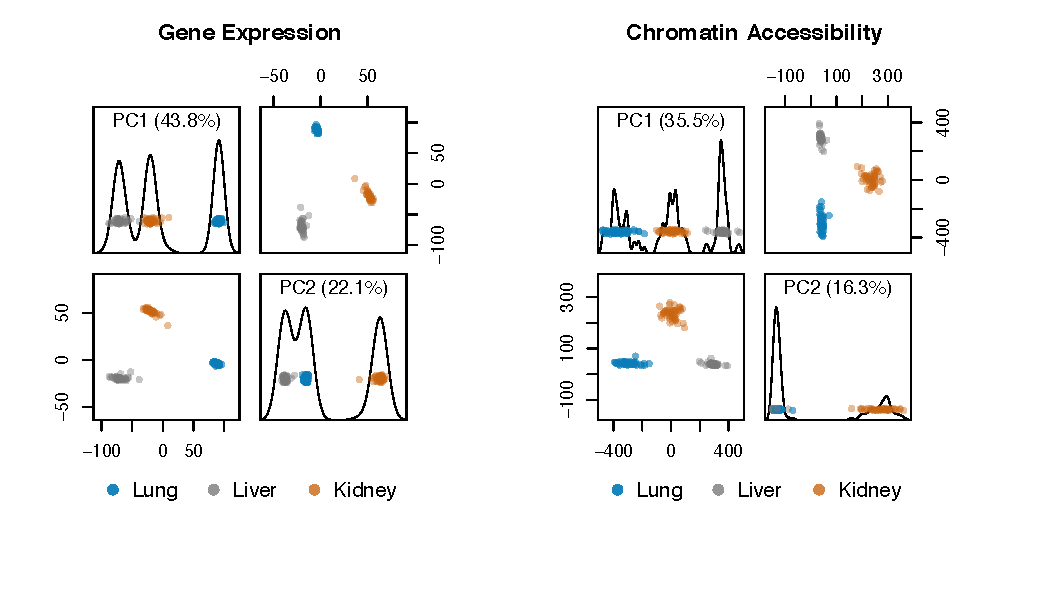
\includegraphics[width=0.8\textwidth, trim={0.25in 0.5in 0.5in 0in}, clip]{figs/pca_plot.pdf}
\caption{\textbf{Principle components analysis identifies tissue type as key source of variation for gene expression and chromatin accessibility.} Molecular traits for lung (blue), liver (gray), and kidney (orange) tissue samples were derived from RNA-seq and ATAC-seq data. Principal components (PC) 1 and 2 capture a majority of the variation and show a greater amount of between tissue variability than within tissue variability. \label{fig:pca_plots}}
\end{figure*}

\begin{figure*}[hp]
\renewcommand{\familydefault}{\sfdefault}\normalfont
\centering
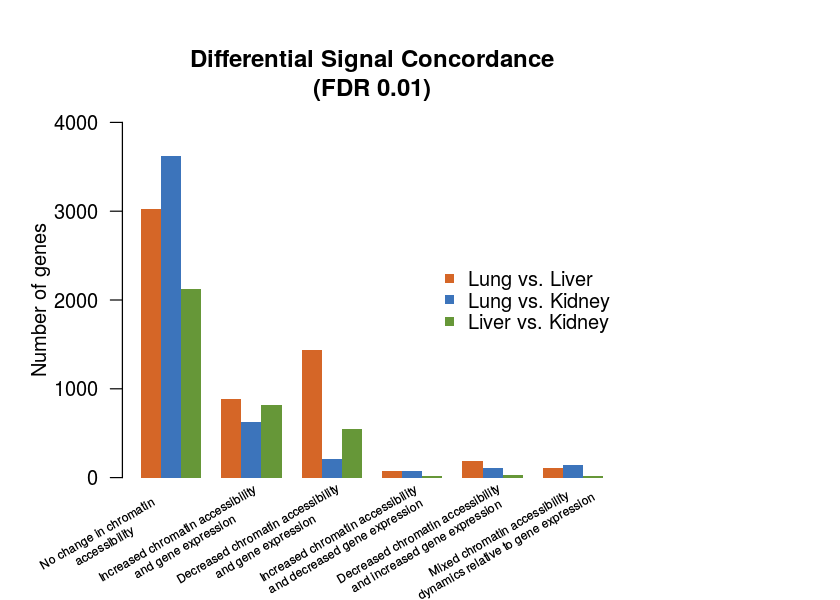
\includegraphics[width=0.8\textwidth, trim={0in 0in 0in 0in}, clip]{figs/diff_concordance.png}
\caption{\textbf{Concordance between differentially expressed (DE) genes and differentially accessible regions (DAR) in between-tissue comparisons.} Genes were categorized by the direction of the difference in expression and chromatin accessibility in their promoter regions.\label{fig:diff_concordance}}
\end{figure*}

\begin{figure*}[hp]
\renewcommand{\familydefault}{\sfdefault}\normalfont
\centering
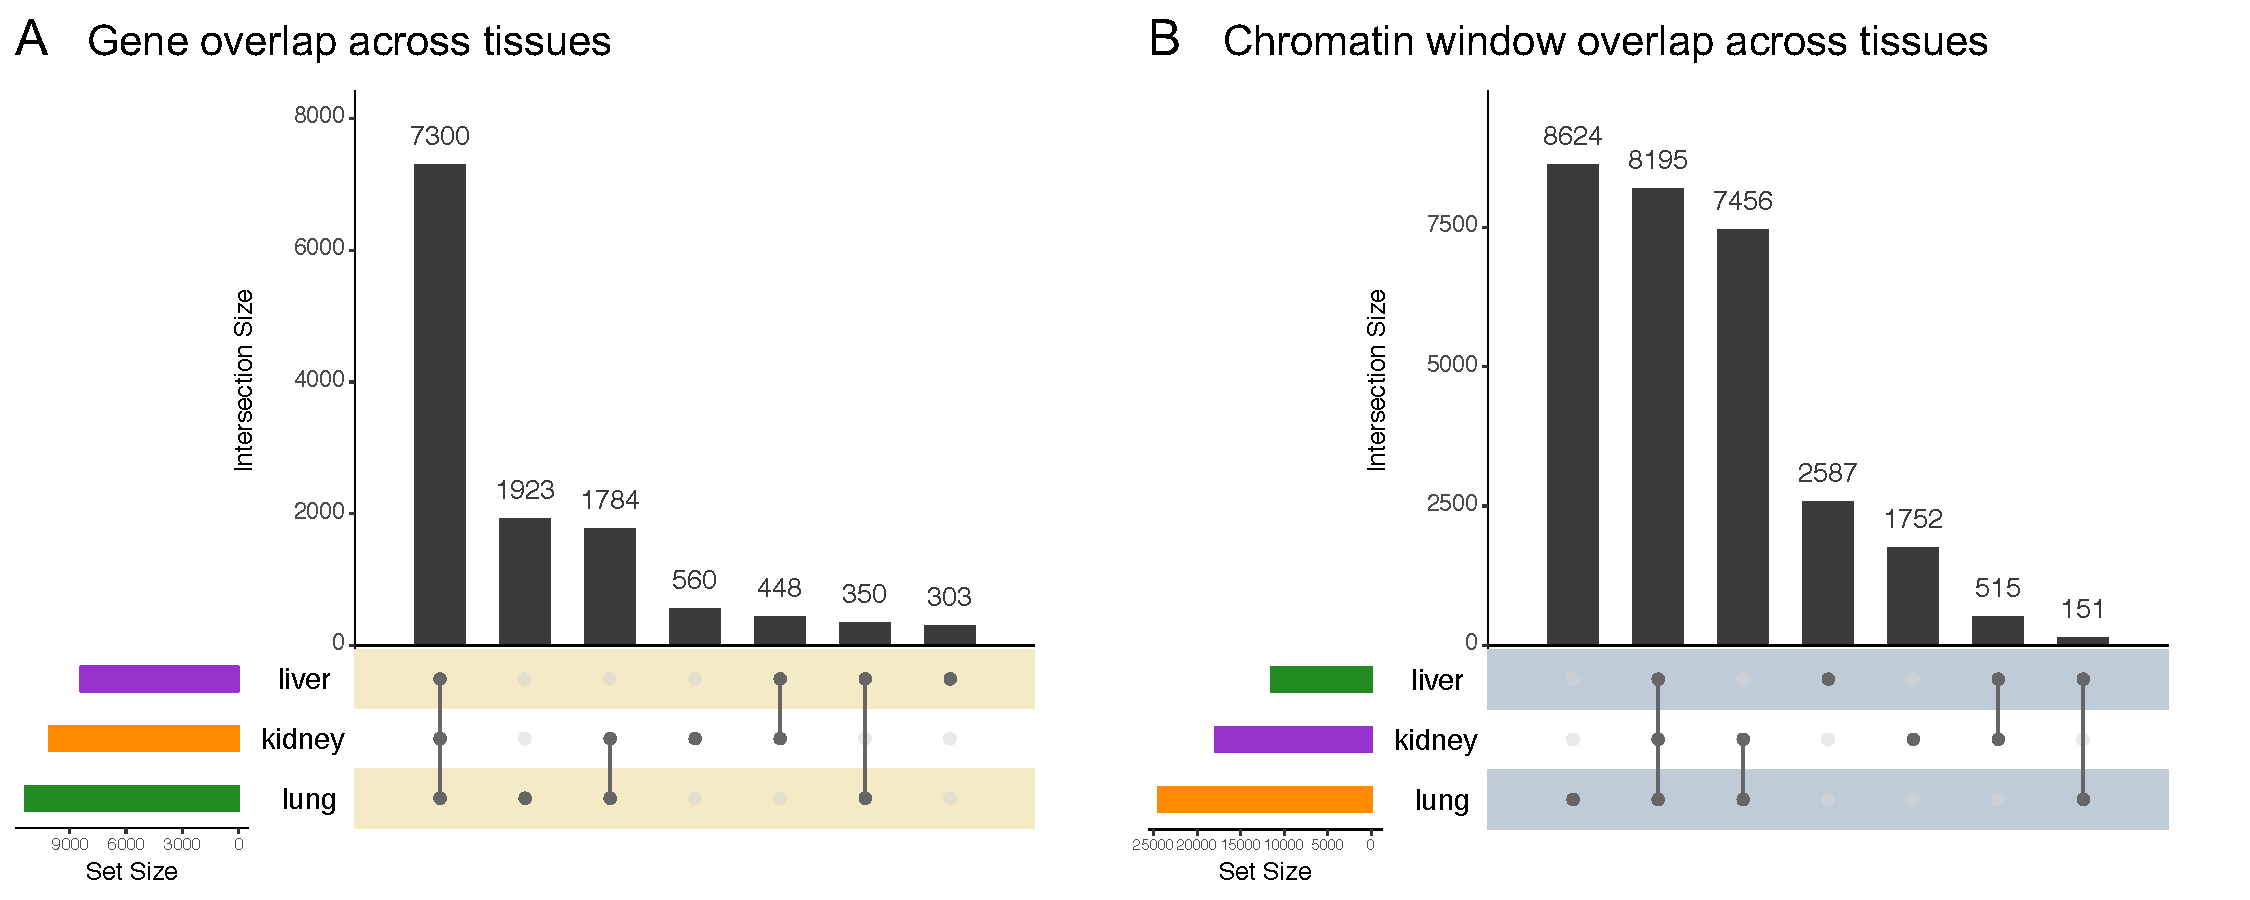
\includegraphics[width=\textwidth, trim={0in 0in 0in 0in}, clip]{figs/upset_genes_chromatin.pdf}
\caption{\textbf{Overlap across tissues of genes and chromatin windows used for QTL analysis.} Sequence traits were filtered to remove outcomes more likely to cause in spurious QTL signal. Genes with TPM $\le 1$ and chromatin windows with TMP $\le 5$ for $\ge$ 50\% of samples were removed from analysis. After this filtering process, lung had the greatest number of traits analyzed, for both genes and chromatin windows, followed by kidney and then liver. 
\label{fig:upset_genes_chromatin}}
\end{figure*}

\begin{figure*}[hp]
\renewcommand{\familydefault}{\sfdefault}\normalfont
\centering
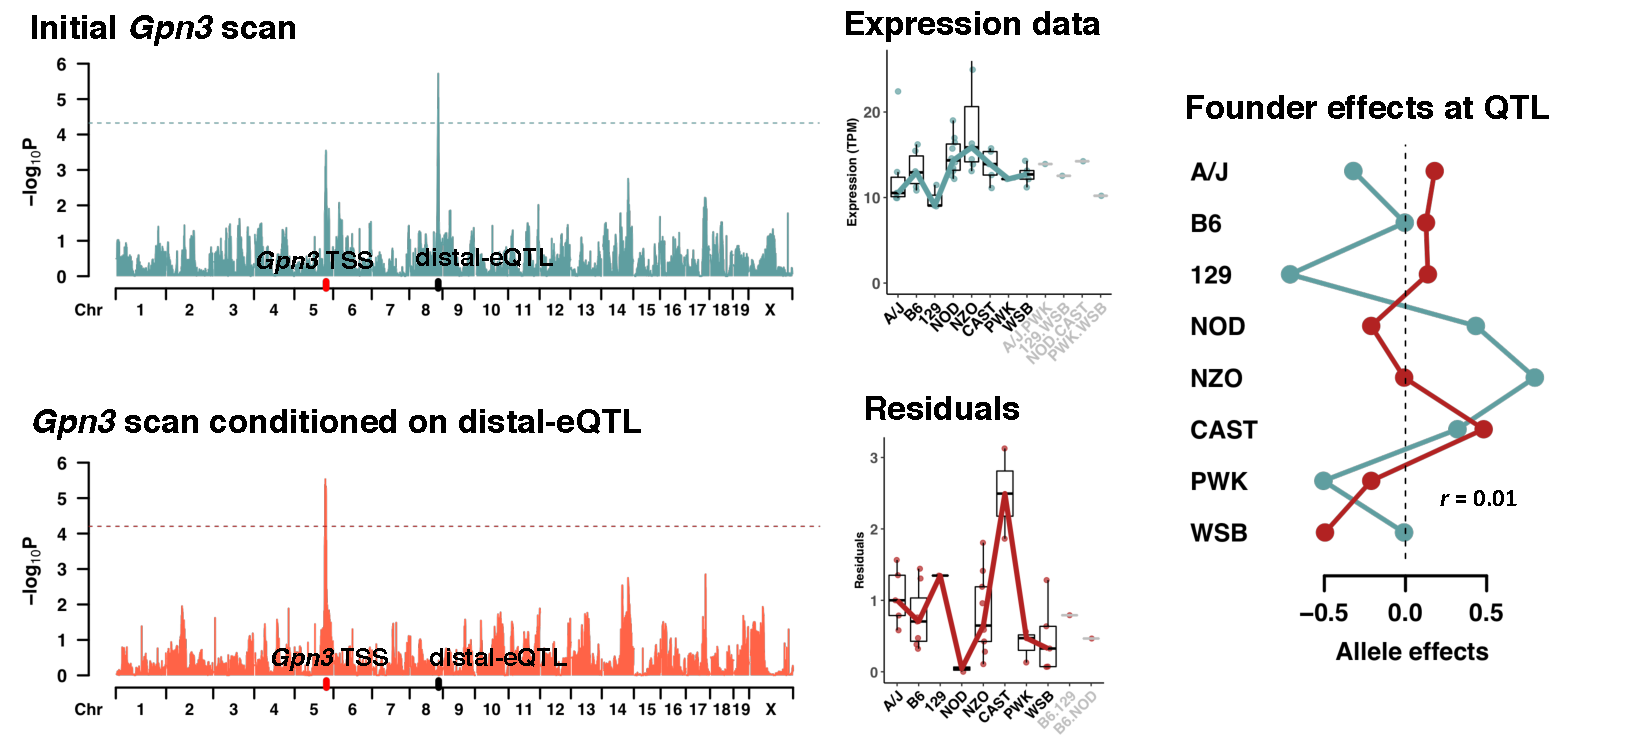
\includegraphics[width=\textwidth, trim={0in 0in 0in 0in}, clip]{figs/gpn3_conditional_scan.pdf}
\caption{\textbf{Detection of local-eQTL after conditioning on distal-eQTL for \textit{Gpn3}.} The multi-stage conditional regression approach of Method 1 allows for the detection of multiple genome-wide significant QTL, which can then be appropriately incorporated into a FDR procedure across many outcomes. In this example in lung tissue, the gene \textit{Gpn3} initially has a strong distal-eQTL on chromosome 8 (A). Though a peak is detected near the TSS of \textit{Gpn3}, it does not meet genome-wide significance. However, after conditioning on the distal-eQTL, the local-eQTL is detected (B). Horizontal dashed lines represent empirical 95\% significance thresholds based on 1000 permutations.
\label{fig:conditional_scans}}
\end{figure*}

\begin{figure*}[hp]
\renewcommand{\familydefault}{\sfdefault}\normalfont
\centering
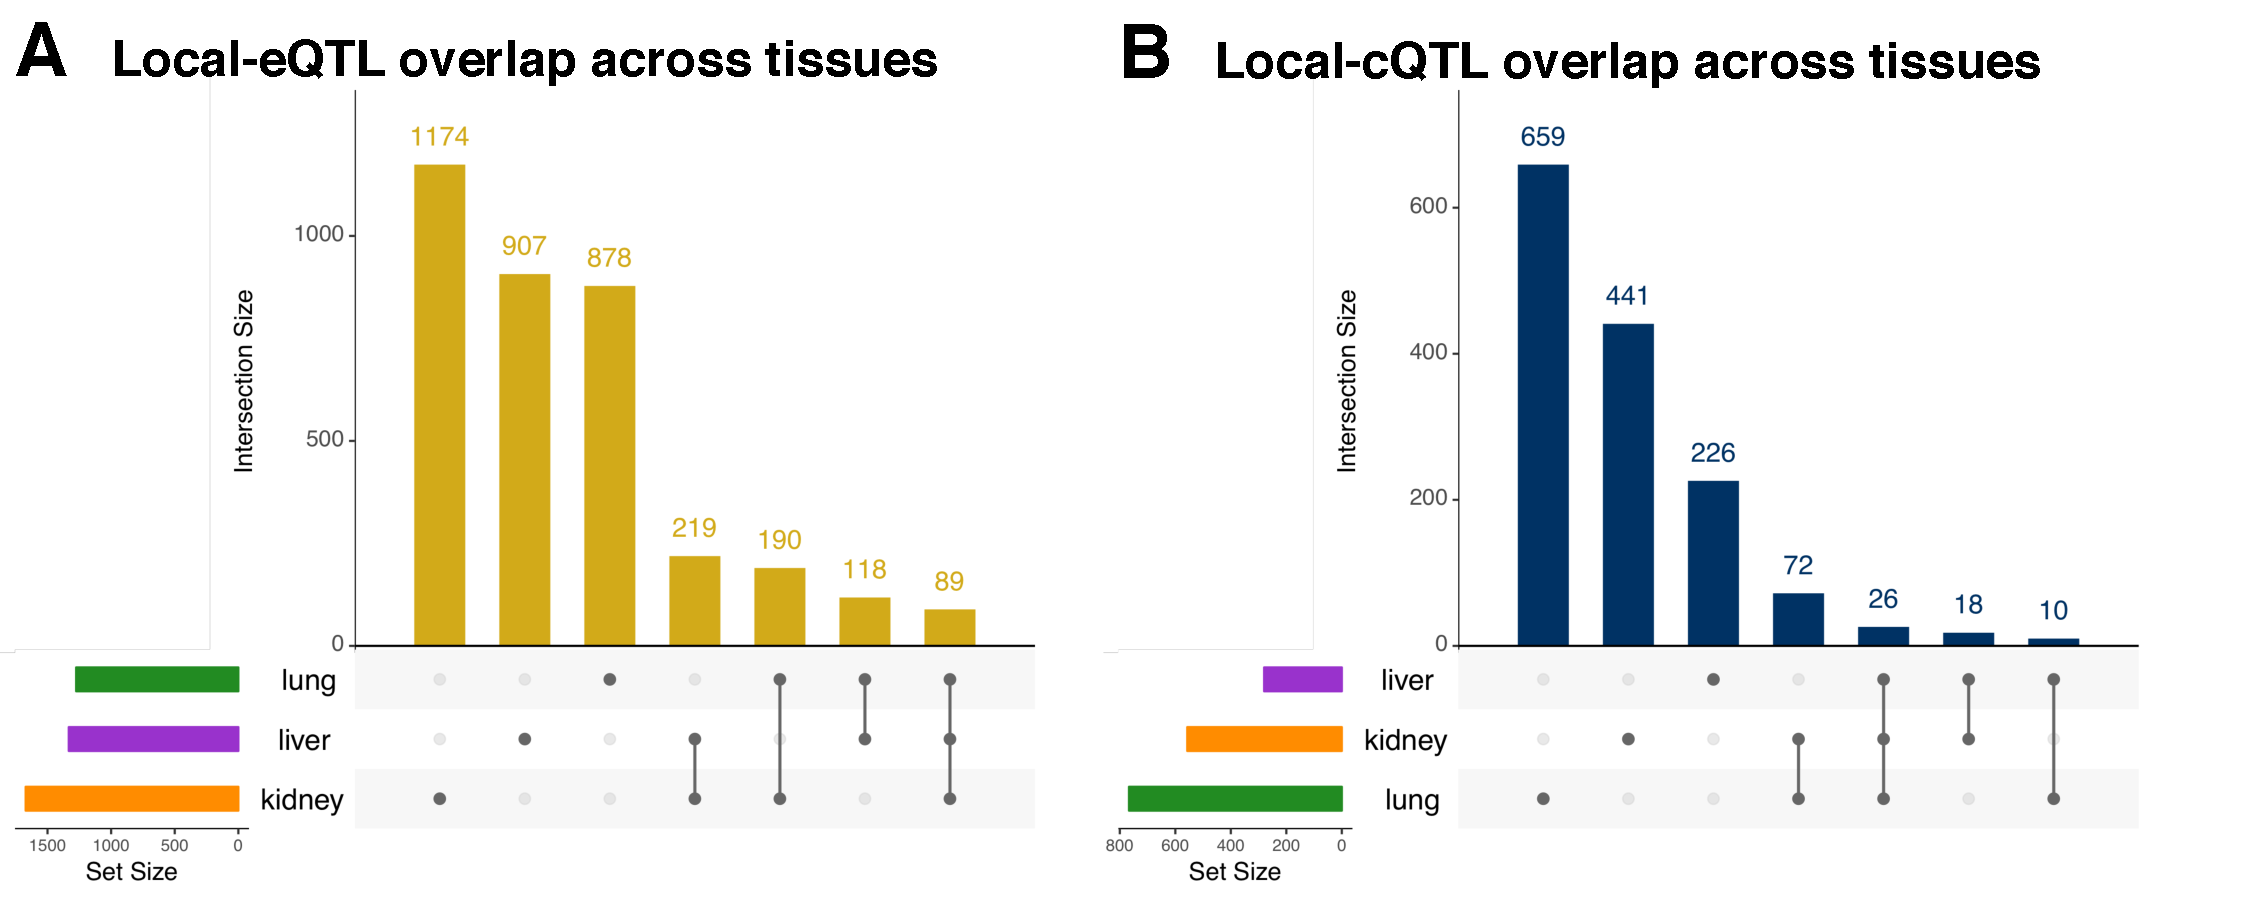
\includegraphics[width=\textwidth, trim={0in 0in 0in 0in}, clip]{figs/upset_eqtl_cqtl.pdf}
\caption{\textbf{Overlap across tissues of genes and chromatin windows with local-QTL detected.} The majority of sequence traits with a local-QTL detected were identified in only a single tissue. Kidney had the highest number of local-eQTL, whereas lung had the highest number of local-cQTL. Liver had a relative lack of local-cQTL, which may relate to its having the fewest chromatin windows analyzed (\textbf{Figure \ref{fig:upset_genes_chromatin} [right]}). Results included local-QTL detected with Method 1 (FDR < 0.1), Method 2 (FDR < 0.1), and Method 3 (genome-wide and chromosome-wide). 
\label{fig:upset_eqtl_cqtl}}
\end{figure*}

\begin{figure*}[h]
\renewcommand{\familydefault}{\sfdefault}\normalfont
\centering
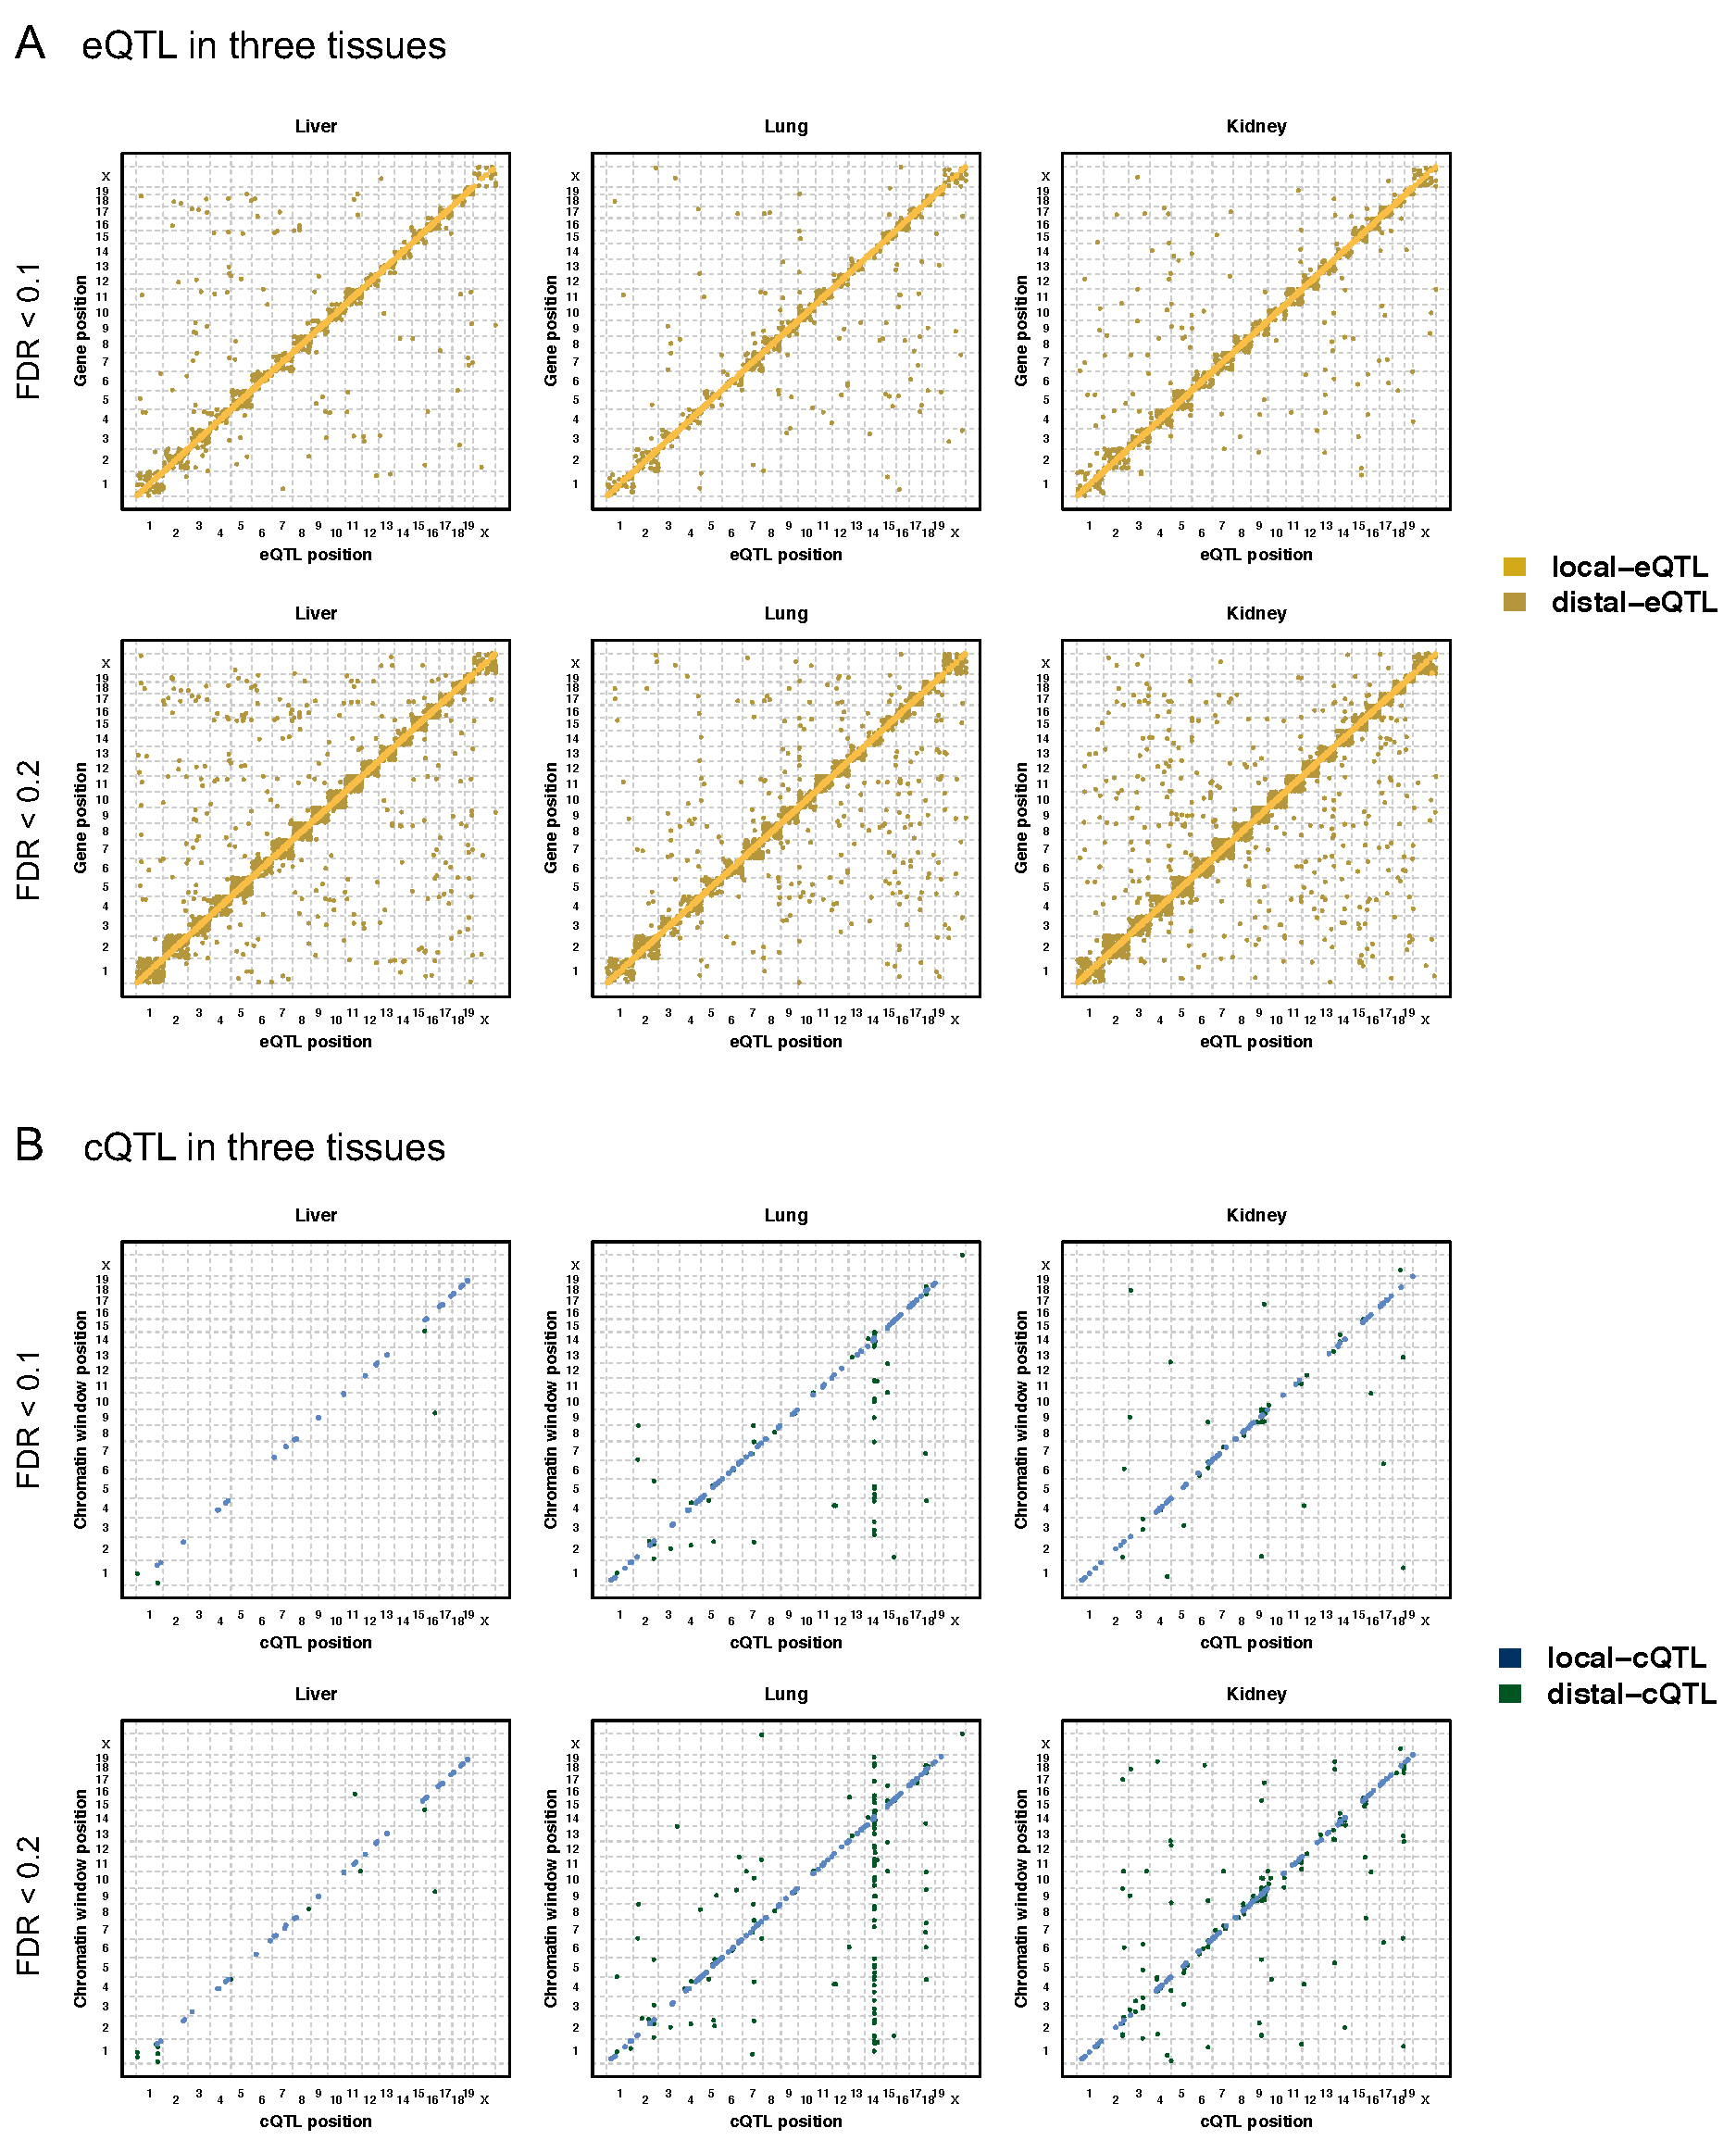
\includegraphics[width=0.8\textwidth, trim={0in 1.5in 0in 0in}, clip]{figs/qtl_map_supplemental.pdf}
\caption{\textbf{QTL mapping results using only Method 1 or Method 2.} QTL map plots of eQTL and cQTL with FDR controlled at 0.1 and 0.2 for liver, lung, and kidney. Detected QTL from Method 1 (multi-stage FDR) and Method 2 (chromosome-wide FDR) are included. Method 2, which uses FDR control for chromosome-wide significant QTL, produces a large number of intra-chromosomal distal QTL. The y-axis represents the genomic position of the gene or chromatin site, and the x-axis represents the genomic position of the QTL. Local-QTL appear as dots along the diagonal.
\label{fig:grid_fdr_plot}}
\end{figure*}

\begin{figure*}[h]
\centering
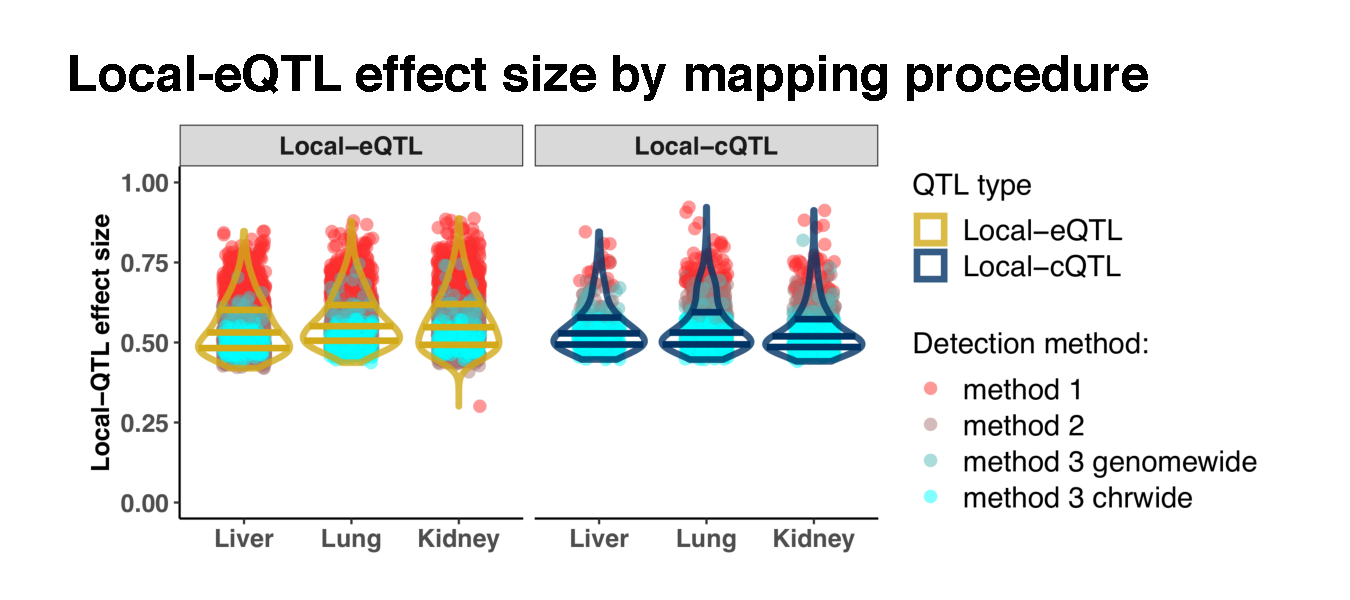
\includegraphics[width=\textwidth, trim={0in 0in 0in 0in}, clip]{figs/qtl_effect_size_by_method.pdf}
\caption{\textbf{Local-QTL effect sizes by mapping procedure.} Statistical procedures with greater rigor have reduced power to detect QTL of smaller effect sizes, shown in liver, lung, and kidney tissues for gene expression (yellow line) and chromatin accessibility (blue line). Each dot represents a detected local-QTL, colored according to the highest stringency mapping procedure that detected it. The three horizontal bars represent the 25\textsuperscript{th}, 50\textsuperscript{th}, and 75\textsuperscript{th} quantiles of QTL effect sizes for all local-QTL per tissue. The multi-stage genome-wide FDR (Method 1) generally detects QTL with effect size > 30\%, whereas the chromosome-wide FDR (Method 2), and FWER-adjusted p-values (permP; Method 3), genome-wide or chromosome-wide can detect QTL effect sizes > 15\%. Effect size estimates correspond to a fixed effects model of the QTL (Eq \ref{eq:effect_size}).
\label{fig:qtl_effect_sizes_by_method}}
\end{figure*}

\begin{figure*}[h]
\centering
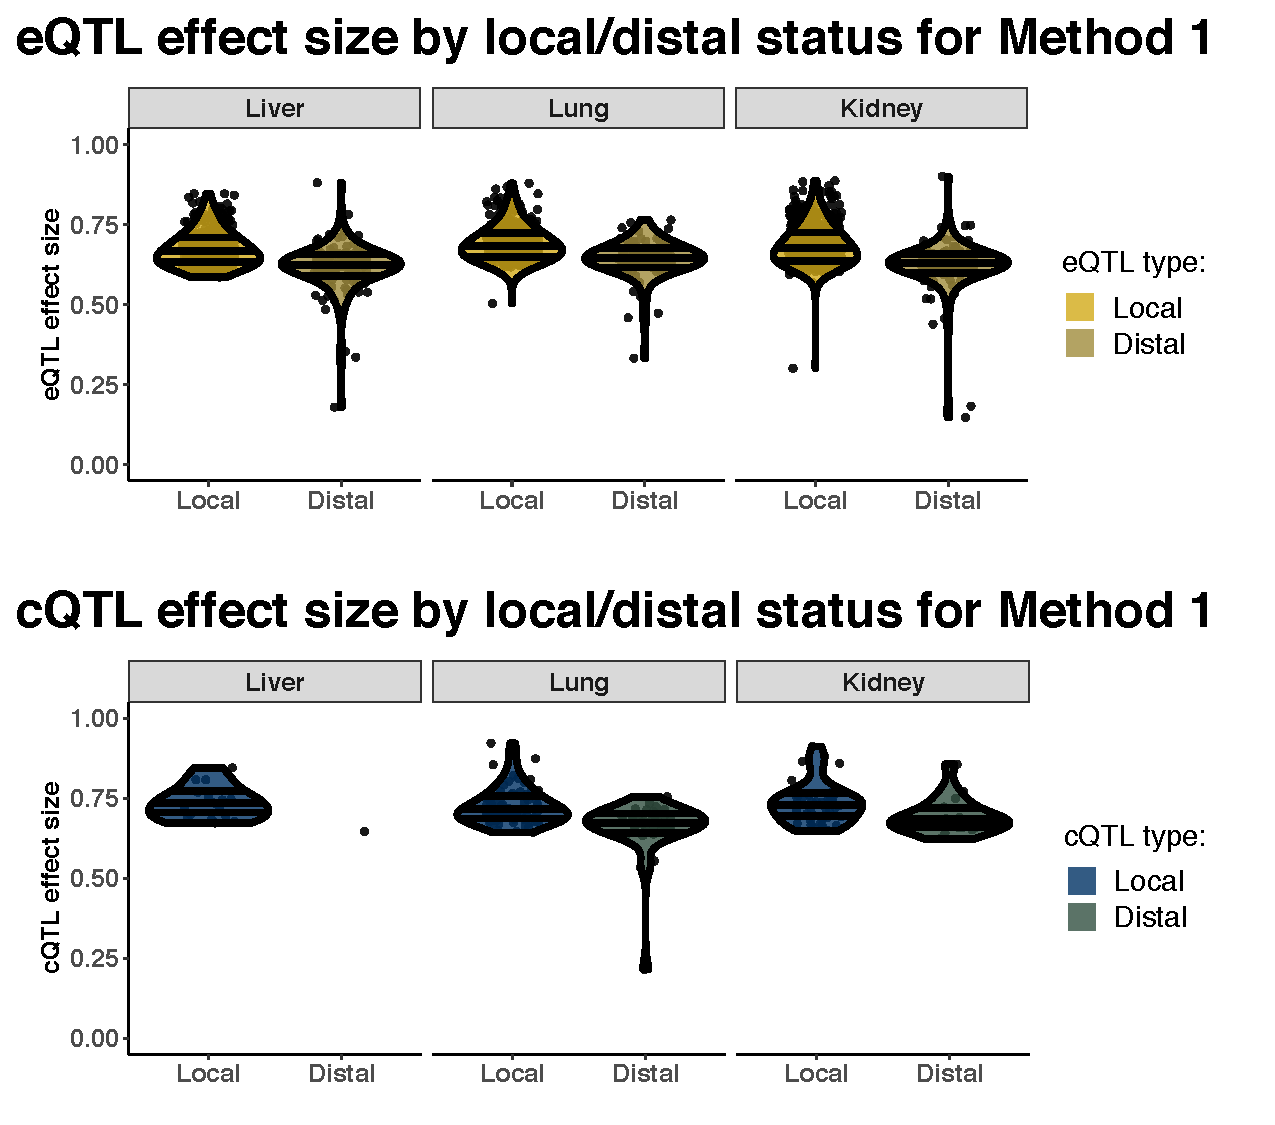
\includegraphics[width=0.9\textwidth, trim={0in 0in 0in 0in}, clip]{figs/qtl_effect_sizes_strict.pdf}
\caption{\textbf{QTL effect sizes by local/distal status for Method 1.} Each dot represents a detected QTL through either Method 1 (FDR $\leq$ 0.1). The three horizontal bars represent the 25\textsuperscript{th}, 50\textsuperscript{th}, and 75\textsuperscript{th} quantiles of QTL effect sizes for all local-QTL per tissue. More local-QTL are detected and have larger effects on average than the detected distal-QTL, in both gene expression and chromatin accessibility. Effect size estimates are based on a fixed effects model (Eq \ref{eq:effect_size}).
\label{fig:qtl_effect_sizes_strict}}
\end{figure*}

\begin{figure*}[h]
\centering
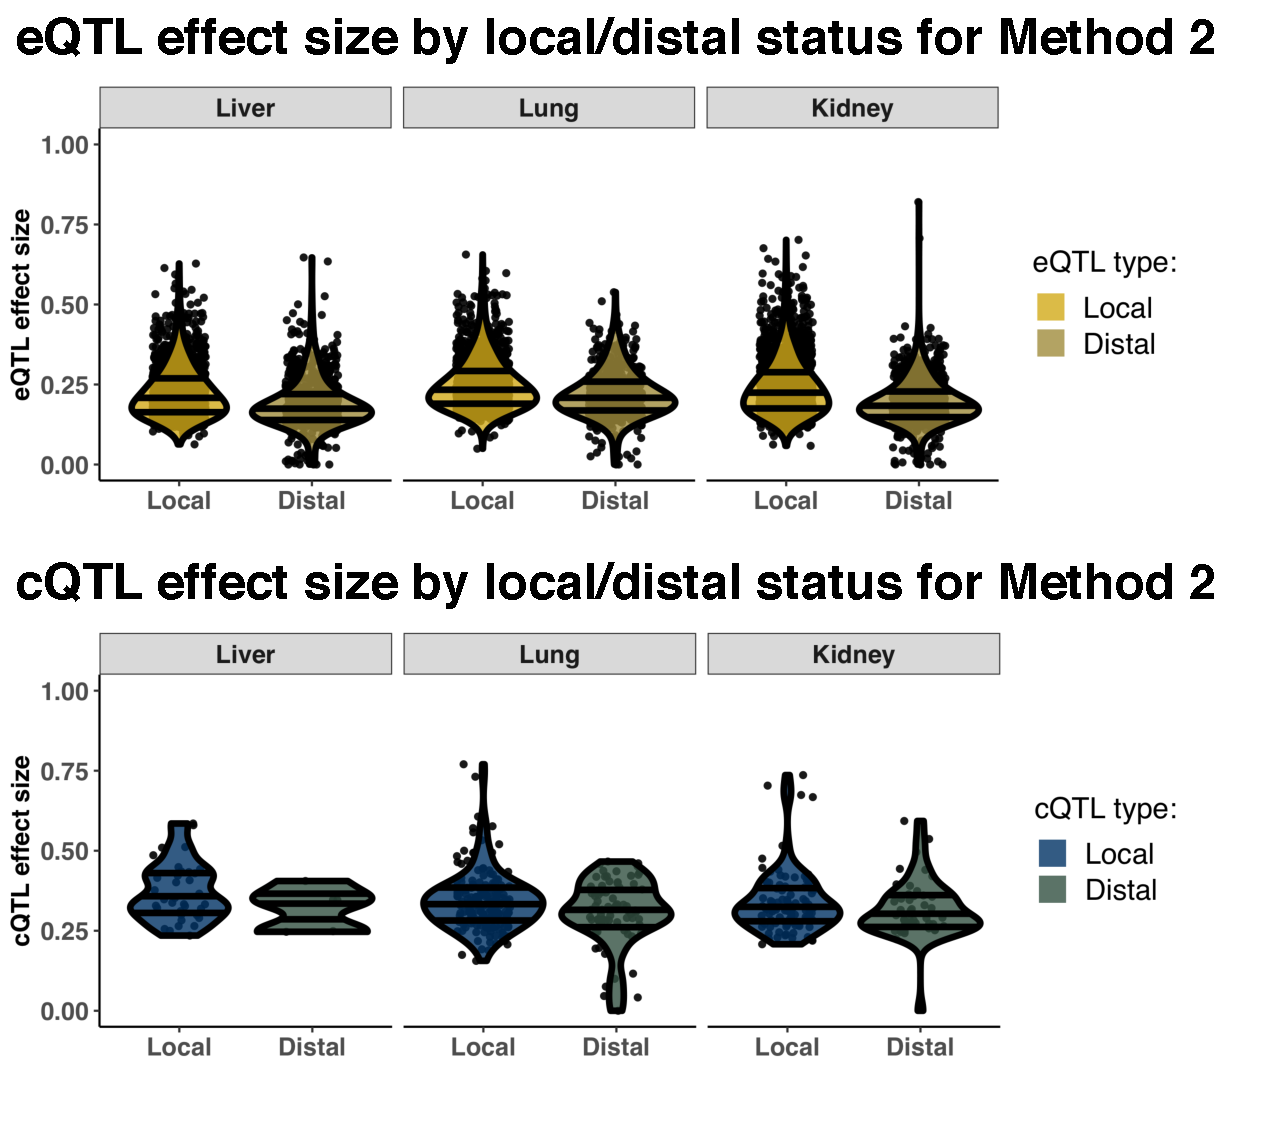
\includegraphics[width=0.9\textwidth, trim={0in 0.25in 0in 0in}, clip]{figs/qtl_effect_sizes_permissive.pdf}
\caption{\textbf{QTL effect sizes by local/distal status for Methods 1 and 2.} Each dot represents a QTL detected through either Method 1 or Method 2 (FDR $\leq$ 0.1). The three horizontal bars represent the 25\textsuperscript{th}, 50\textsuperscript{th}, and 75\textsuperscript{th} quantiles of QTL effect sizes for all local-QTL per tissue. Consistent with Method 1 results, more local-eQTL are detected and have higher effects than distal-QTL. Method 2 detects a large number of intra-chromosomal distal-QTL that Method 1 does not, many of which have low effect sizes. Effect size estimates are based on a fixed effects model (Eq \ref{eq:effect_size}).
\label{fig:qtl_effect_sizes_permissive}}
\end{figure*}

\begin{figure*}[h]
\centering
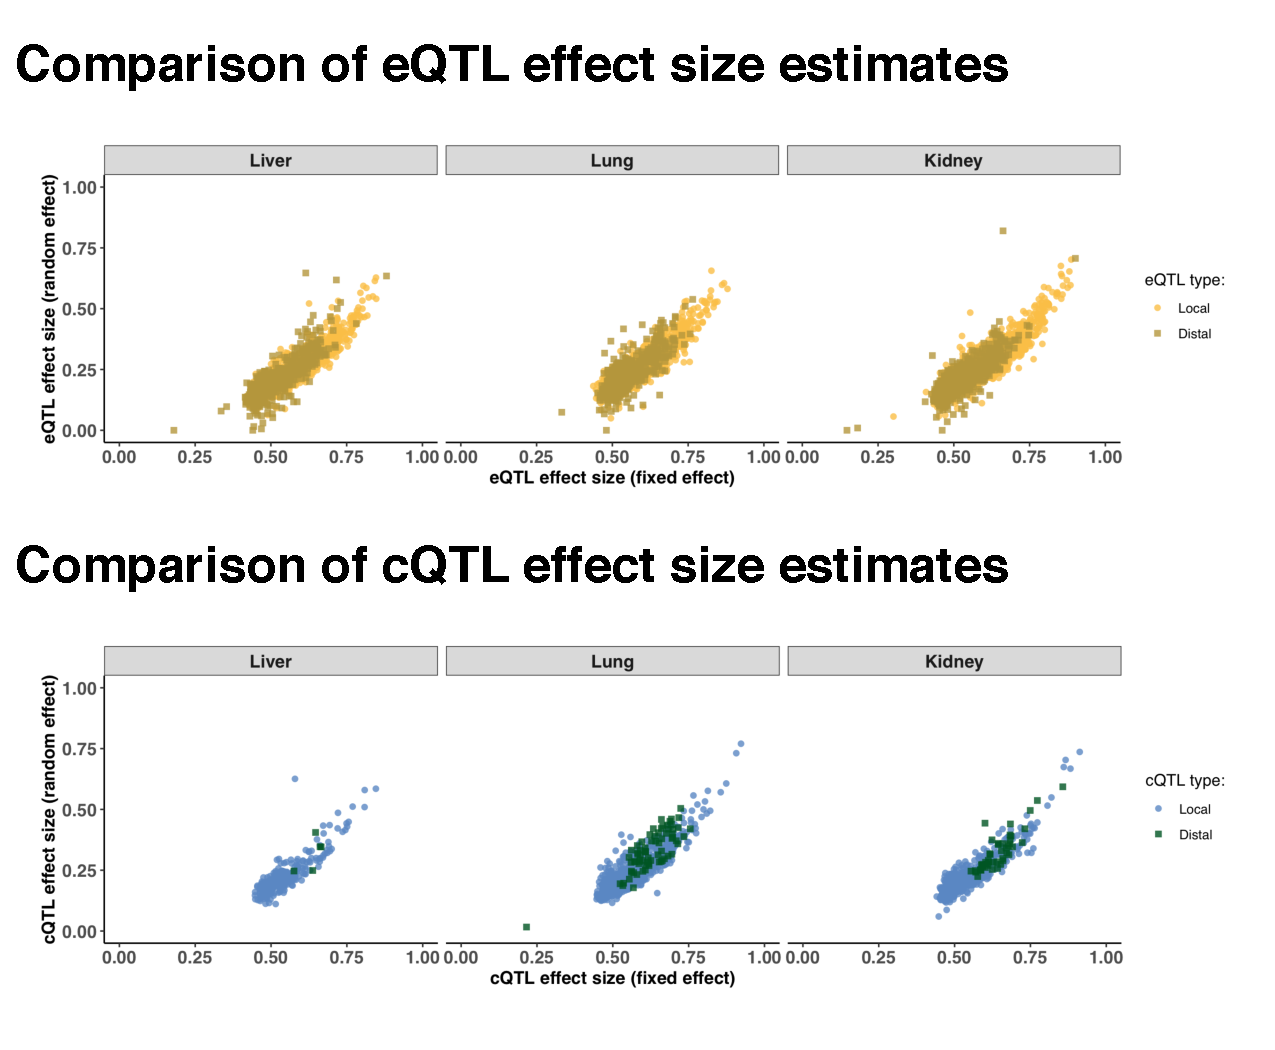
\includegraphics[width=0.9\textwidth, trim={0in 0in 0in 0in}, clip]{figs/fixefvsranef_qtl.pdf}
\caption{\textbf{Comparison of QTL effect sizes estimates from fixed effects and random effects models.} The effect size corresponding to the random effect fit (Y-axis; Eq \ref{eq:effect_size_ranef}) is harshly penalized compared to the fixed effect estimate (X-axis; Eq \ref{eq:effect_size}), likely due to a small sample size of 47 individuals. Notably, there are a number of distal-eQTL that are more harshly reduced by the random effects model compared to the other QTL, likely representing signals resulting from extreme observations or imbalances in founder contributions at the locus. QTL detected by Methods 1 (FDR $\le 0.1$), 2 (FDR $\le 0.1$), and 3 are shown.
\label{fig:qtl_effect_size_fixefvsranef}}
\end{figure*}

\begin{figure*}[hp]
\renewcommand{\familydefault}{\sfdefault}\normalfont
\centering
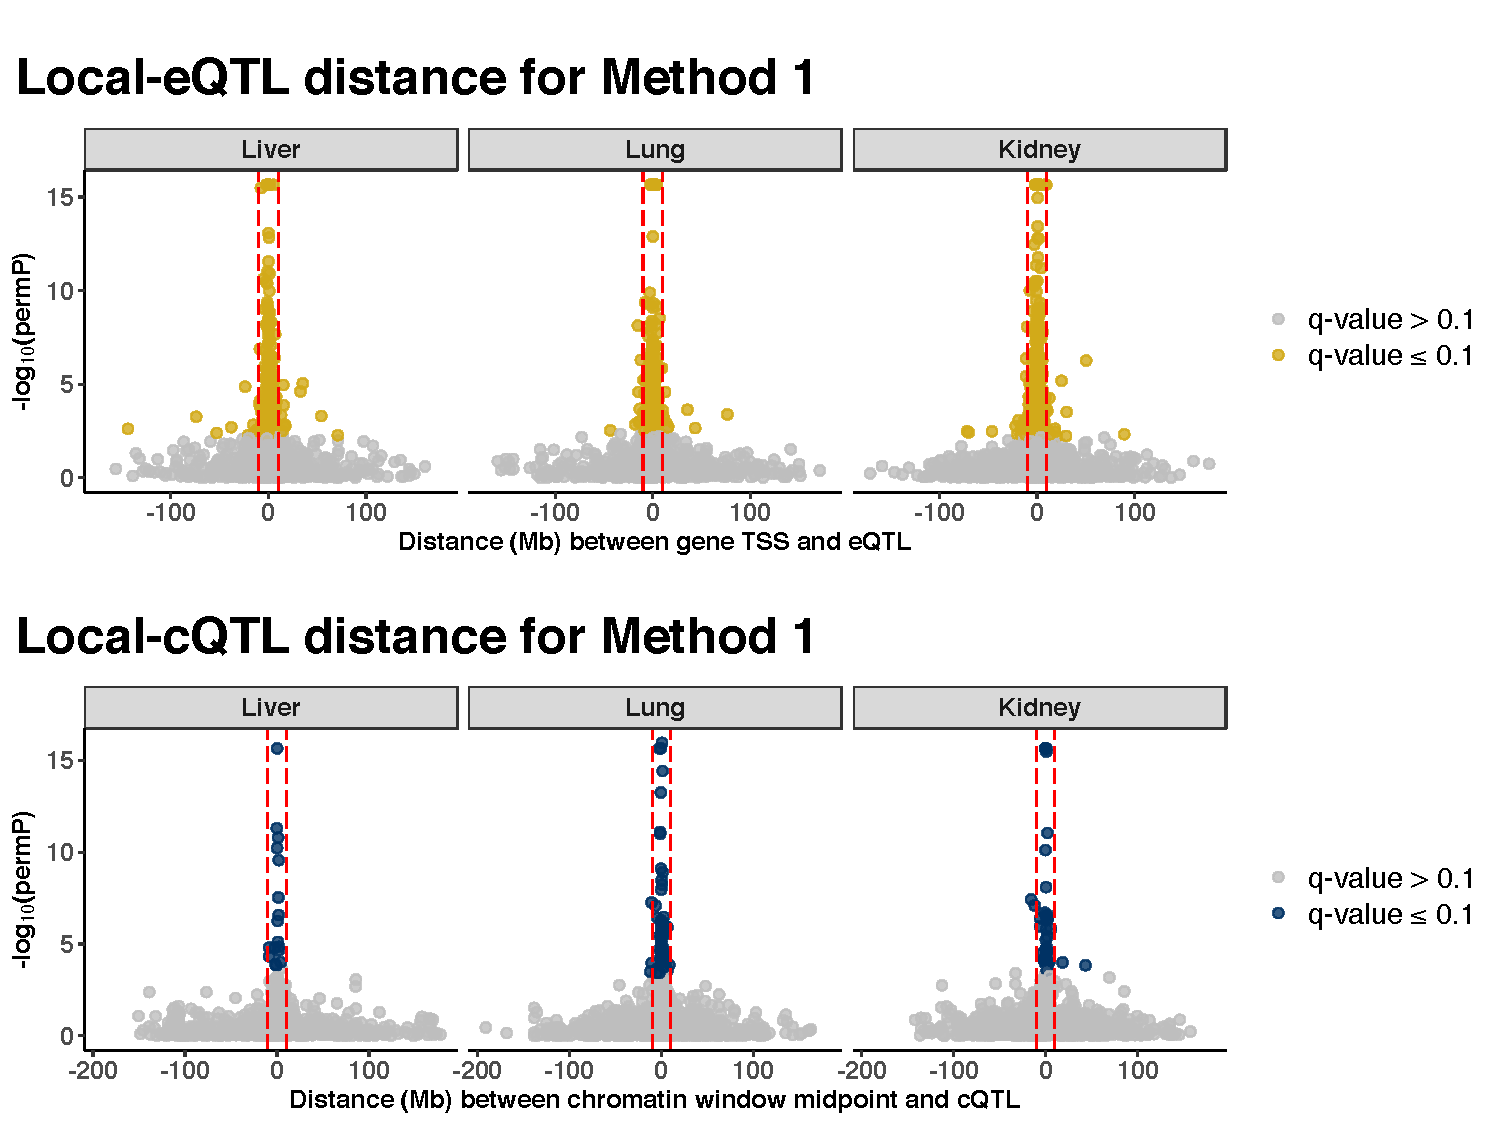
\includegraphics[width=0.9\textwidth]{figs/qtl_distance_method1.pdf}
\caption{\textbf{Highly significant QTL are proximal to gene TSS and chromatin window midpoint.} The genome-wide permutation-based p-value (permP) from Method 1 (first stage-only) for eQTL and cQTL compared to the distance (Mb) from the gene TSS and the midpoint of the chromatin site, respectively. Inter-chromosomal distal-QTL are not included. The red dashed lines represent 10 Mb upstream and downstream of the gene TSS or the midpoint of the chromatin site for classifying QTL as local or distal. Significant signals (yellow or blue), based on $\text{q-value} \le 0.1$, are largely local. \label{fig:genomewide_dist}}
\end{figure*}

\begin{figure*}[hp]
\renewcommand{\familydefault}{\sfdefault}\normalfont
\centering
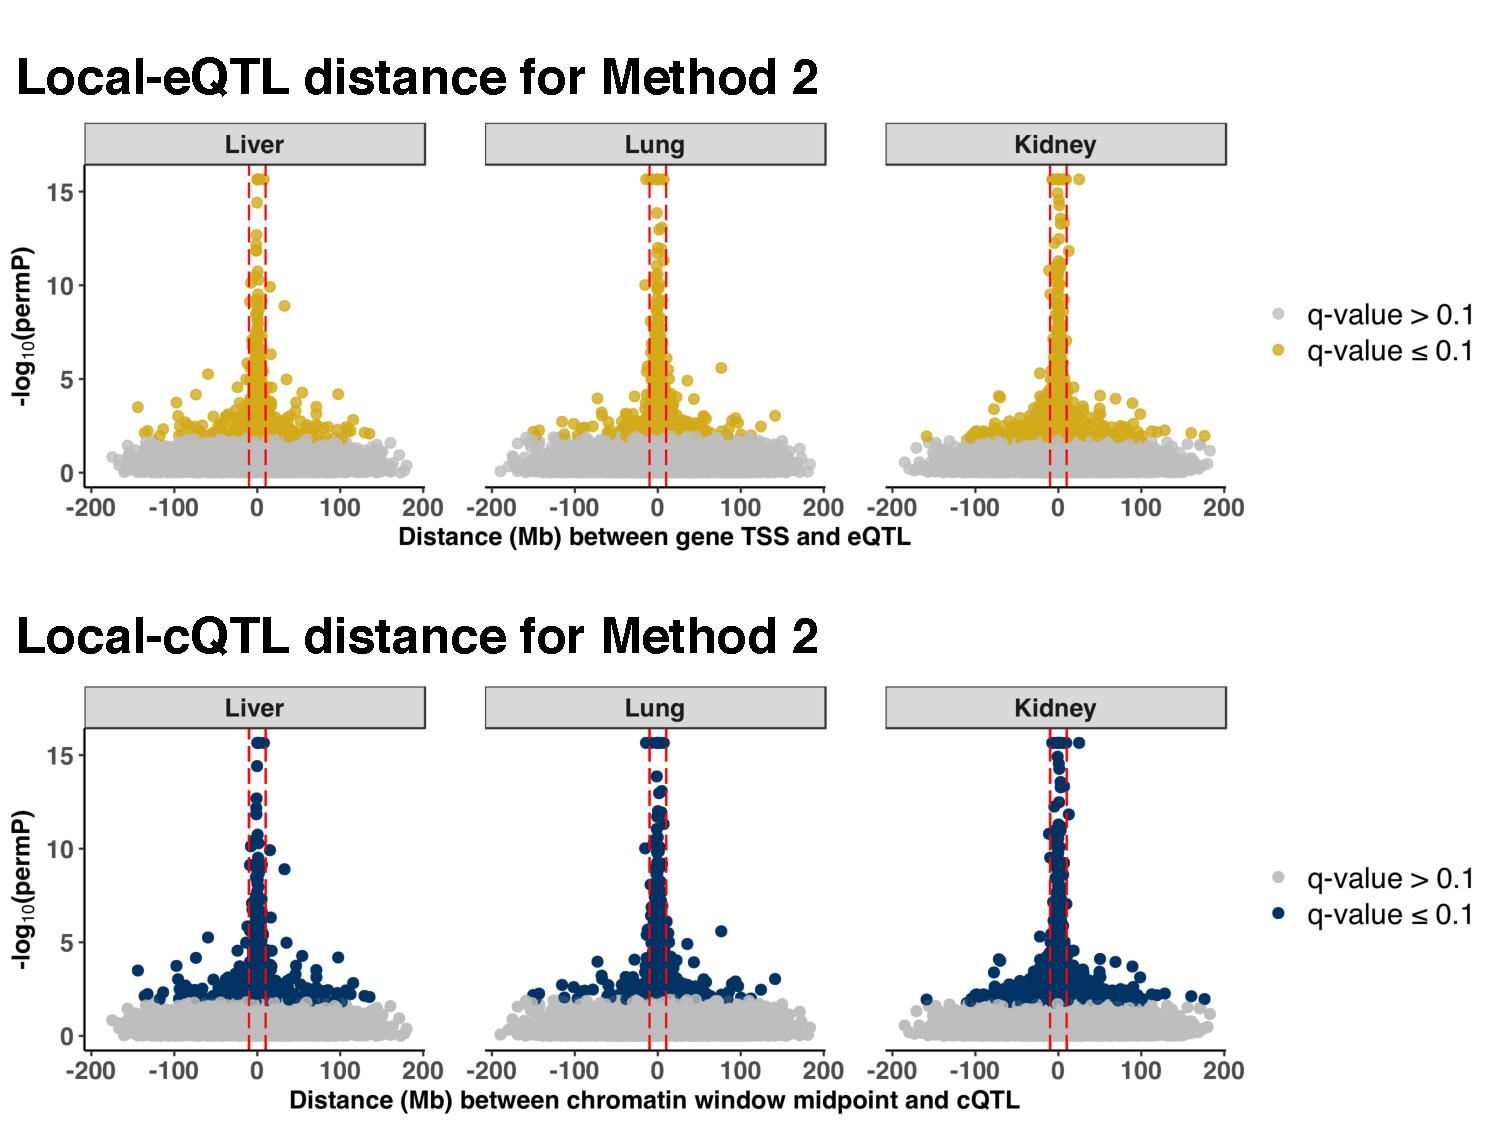
\includegraphics[width=0.9\textwidth]{figs/qtl_distance_method2.pdf}
\caption{\textbf{Methods that use chromosome-wide significance detect many putative intra-chromosomal distal-QTL.} The chromosome-wide permutation-based p-value (permP) from Method 2 for eQTL and cQTL compared to distance (Mb) from the gene TSS and the midpoint of the chromatin site, respectively. Method 2 is restricted to QTL on the local-chromosome. The red dashed lines represent 10 Mb upstream and downstream of gene TSS or chromatin site for classifying an association as local or distal. Significant QTL (yellow or blue) are largely proximal.
\label{fig:chrwide_dist}}
\end{figure*}

\begin{figure*}[hp]
\renewcommand{\familydefault}{\sfdefault}\normalfont
\centering
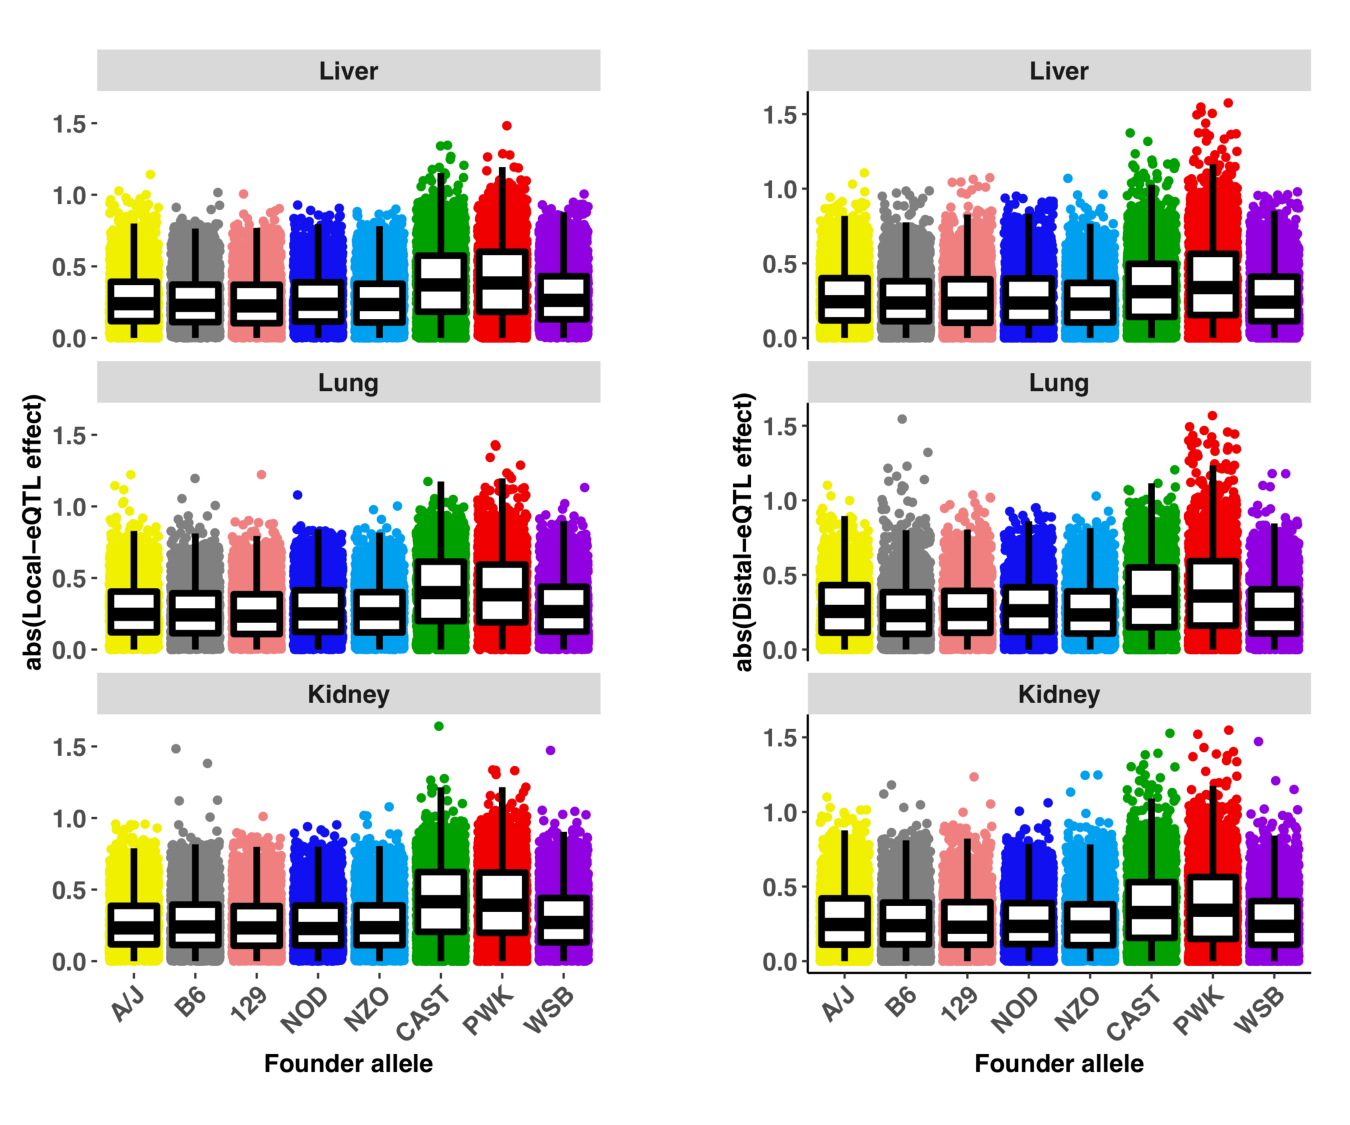
\includegraphics[width=\textwidth, trim={0in 0in 0in 0in}, clip]{figs/all_eqtl_effects_abs.pdf}
\caption{\textbf{CAST and PWK alleles have more extreme effects for eQTL than the other strains.} Founder strain effects were estimated by fitting the QTL effect as a random effect in the model from Eq \ref{eq:alternative_model}, thus representing constrained BLUPs. Each eQTL represents an 8-element effect vector. The founders effects by definition are centered around 0. Taking the absolute value allows for a comparison of the relative magnitudes, allowing for the identification of founders that produce more extreme effects on average. Founder effects for cQTL are displayed in \textbf{Figure \ref{fig:cqtl_effects_abs}}.
\label{fig:eqtl_effects_abs}}
\end{figure*}

\begin{figure*}[hp]
\renewcommand{\familydefault}{\sfdefault}\normalfont
\centering
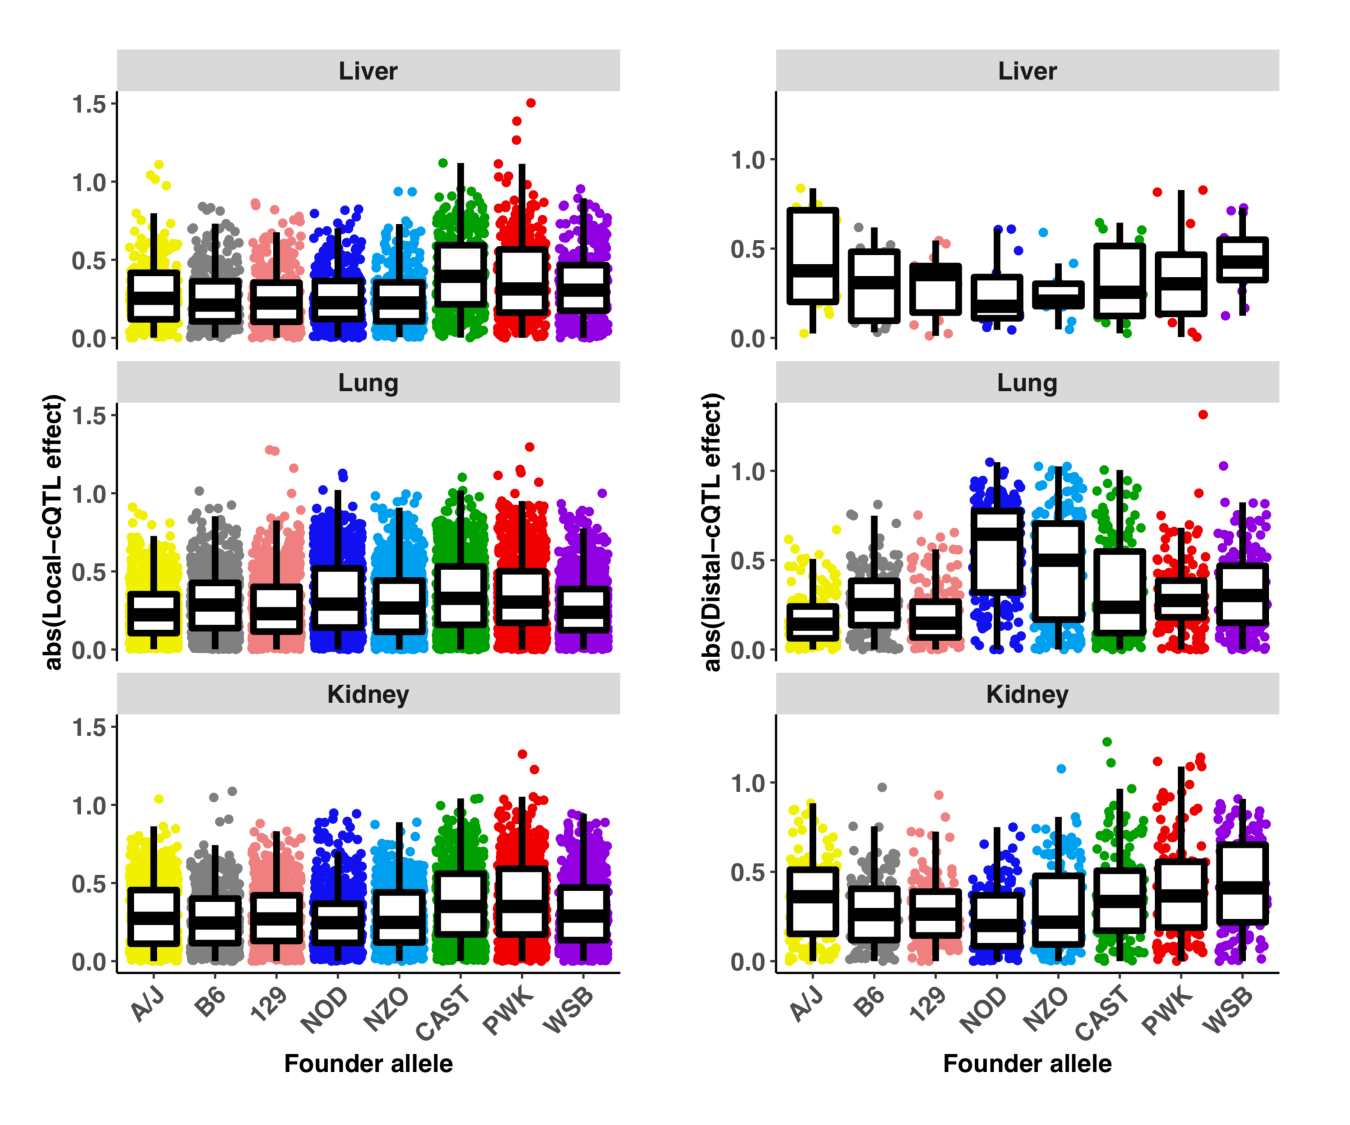
\includegraphics[width=\textwidth, trim={0in 0in 0in 0in}, clip]{figs/all_cqtl_effects_abs.pdf}
\caption{\textbf{CAST and PWK alleles have more extreme effects for cQTL than the other strains.} Using a random effects model to fit the QTL effect in Eq \ref{eq:alternative_model}, founder effects were estimated as BLUPs, which are constrained and centered around 0. Each cQTL is represented by an 8-element effect vector. Founders with on average more extreme effects are identified by comparing the absolute values of effects. Founder effects for eQTL are in \textbf{Figure \ref{fig:eqtl_effects_abs}}, which are similar to cQTL but better represented.
\label{fig:cqtl_effects_abs}}
\end{figure*}

\begin{figure*}[hp]
\renewcommand{\familydefault}{\sfdefault}\normalfont
\centering
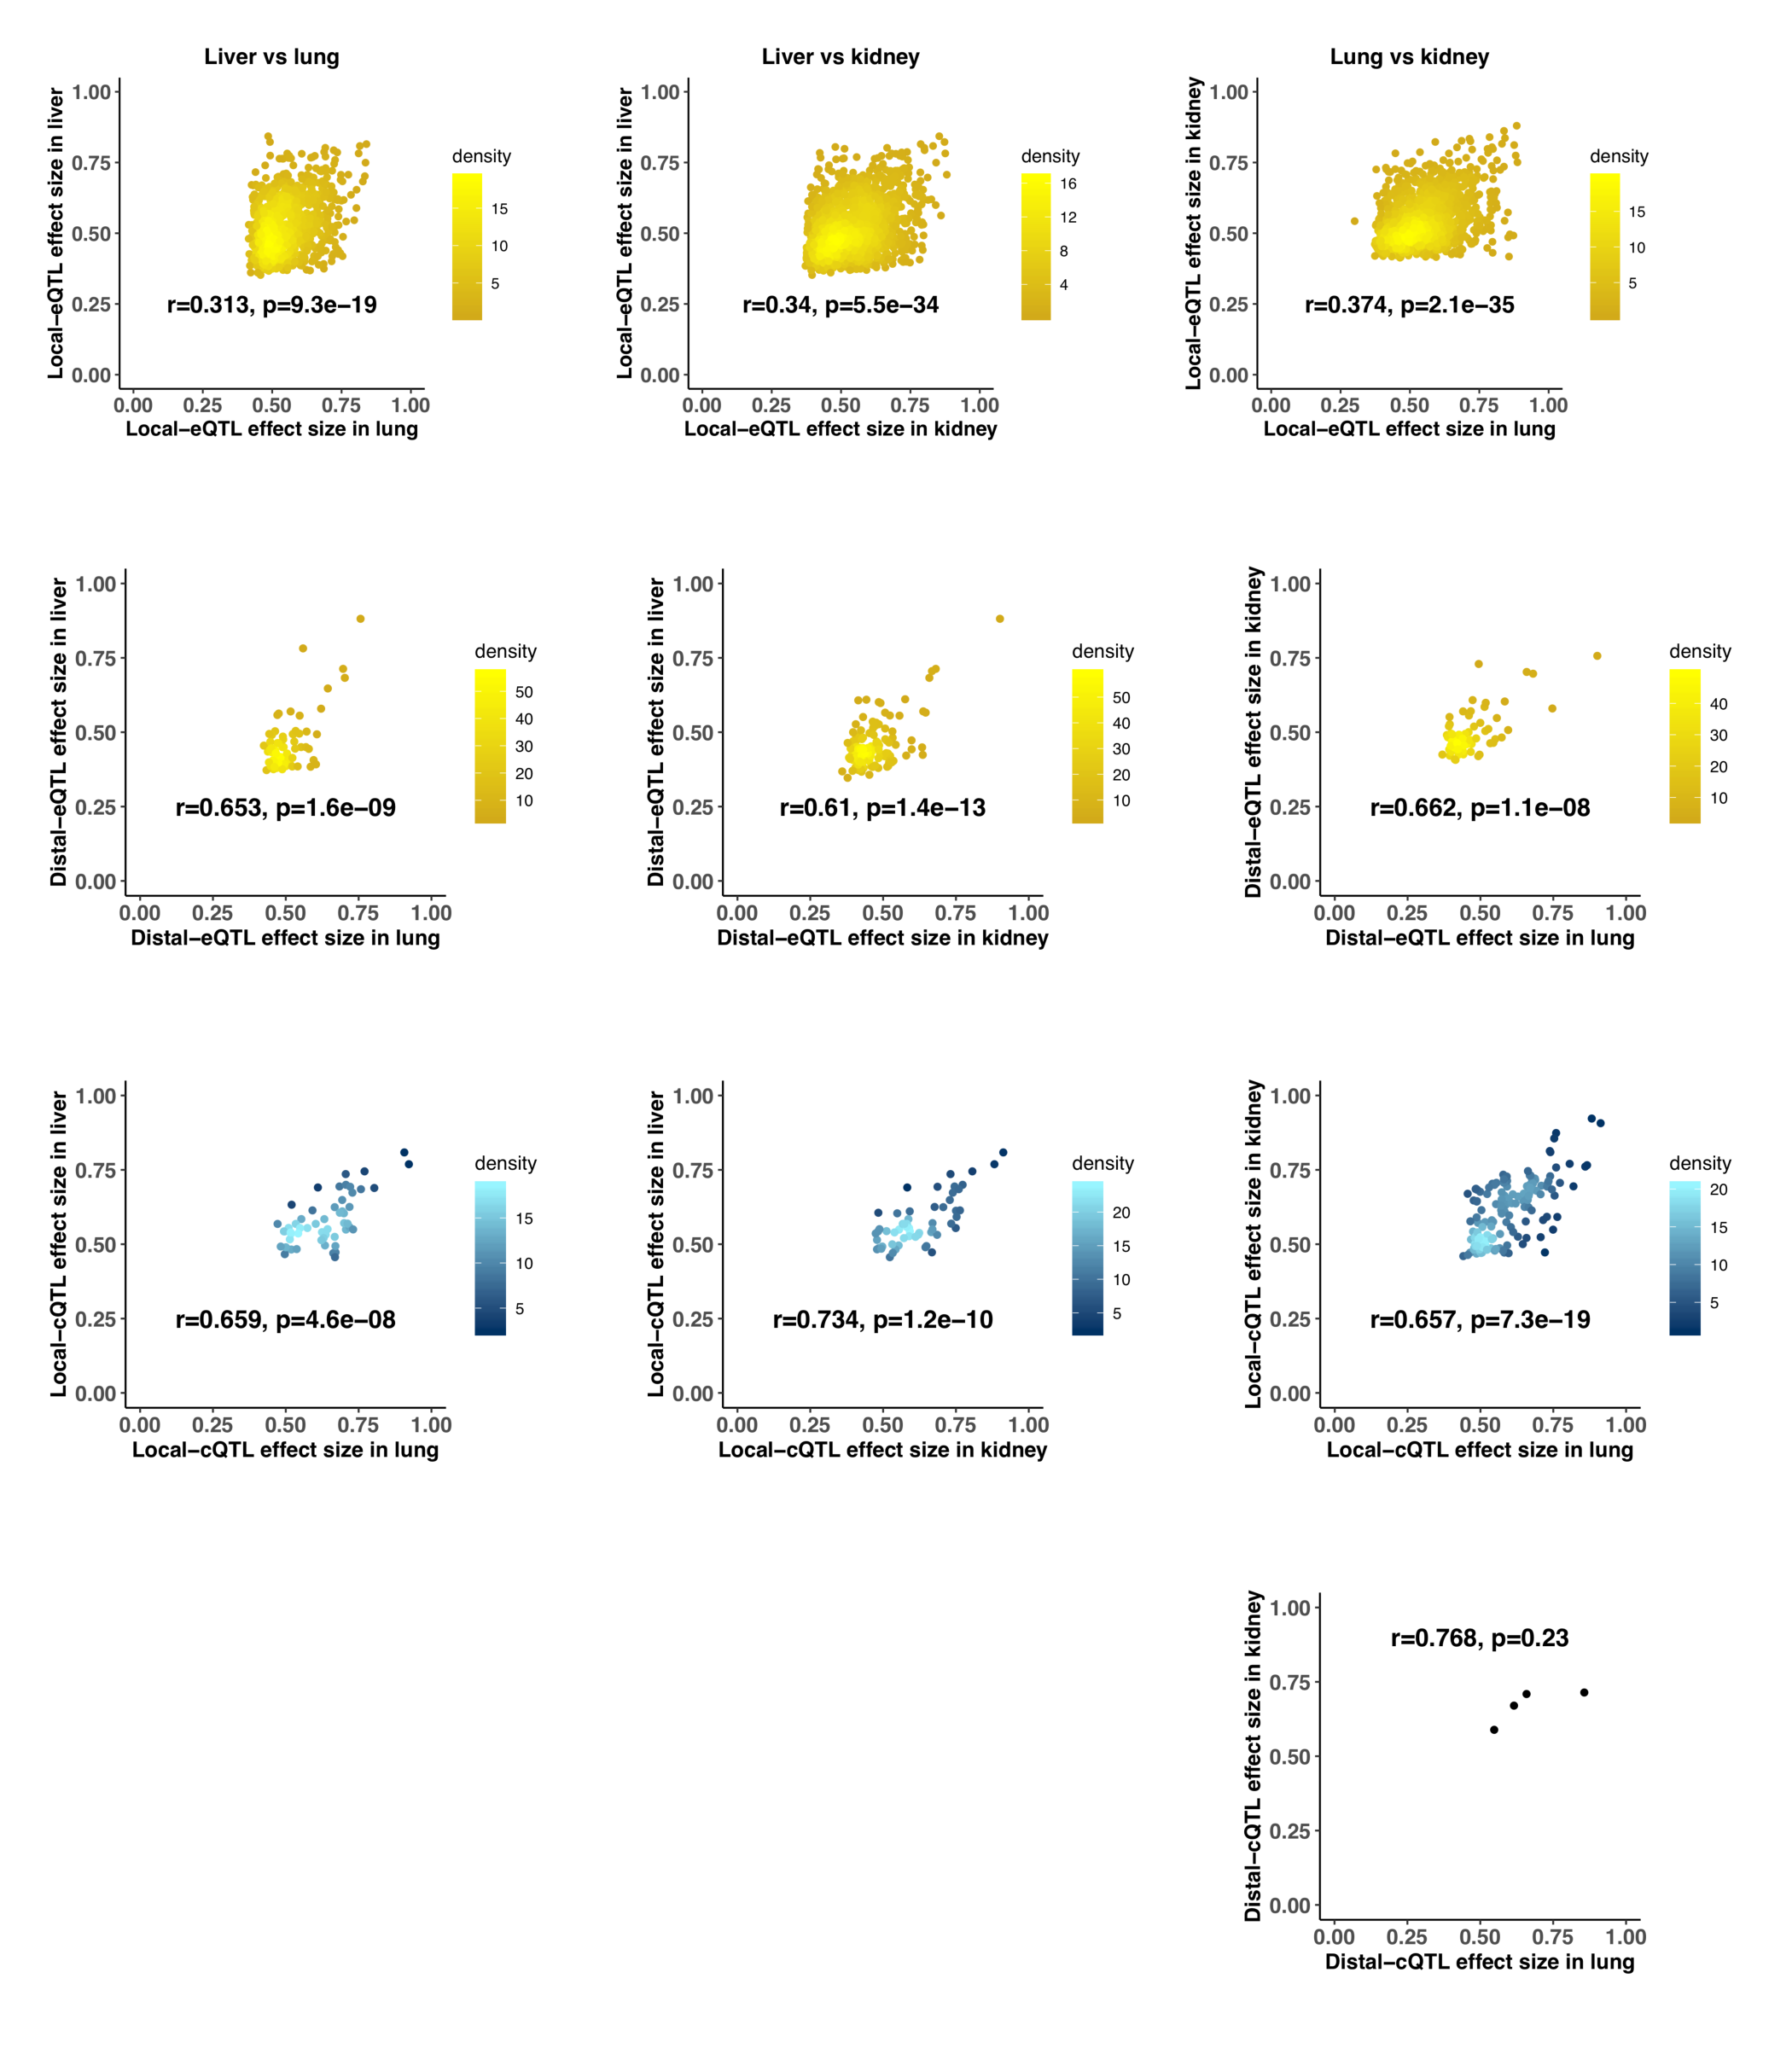
\includegraphics[width=0.9\textwidth, trim={0in 0in 0in 0in}, clip]{figs/effect_size_by_effect_size.pdf}
\caption{\textbf{Effect sizes between QTL pairs are lowly but significantly correlated.} Comparisons of QTL effects sizes, calculated according to Eq \ref{eq:effect_size}, between (liver/lung) are in the left column, (liver/kidney) middle column, and (lung/kidney) right column. eQTL are yellow and cQTL are blue. Local-eQTL are plotted in the top row, distal-eQTL in the second row, local-cQTL in the third row, and distal-cQTL in the bottom row, with only four pairs detected in (lung/kidney). 
\label{fig:qtl_effect_size_comparison}}
\end{figure*}

\begin{figure*}[hp]
\renewcommand{\familydefault}{\sfdefault}\normalfont
\centering
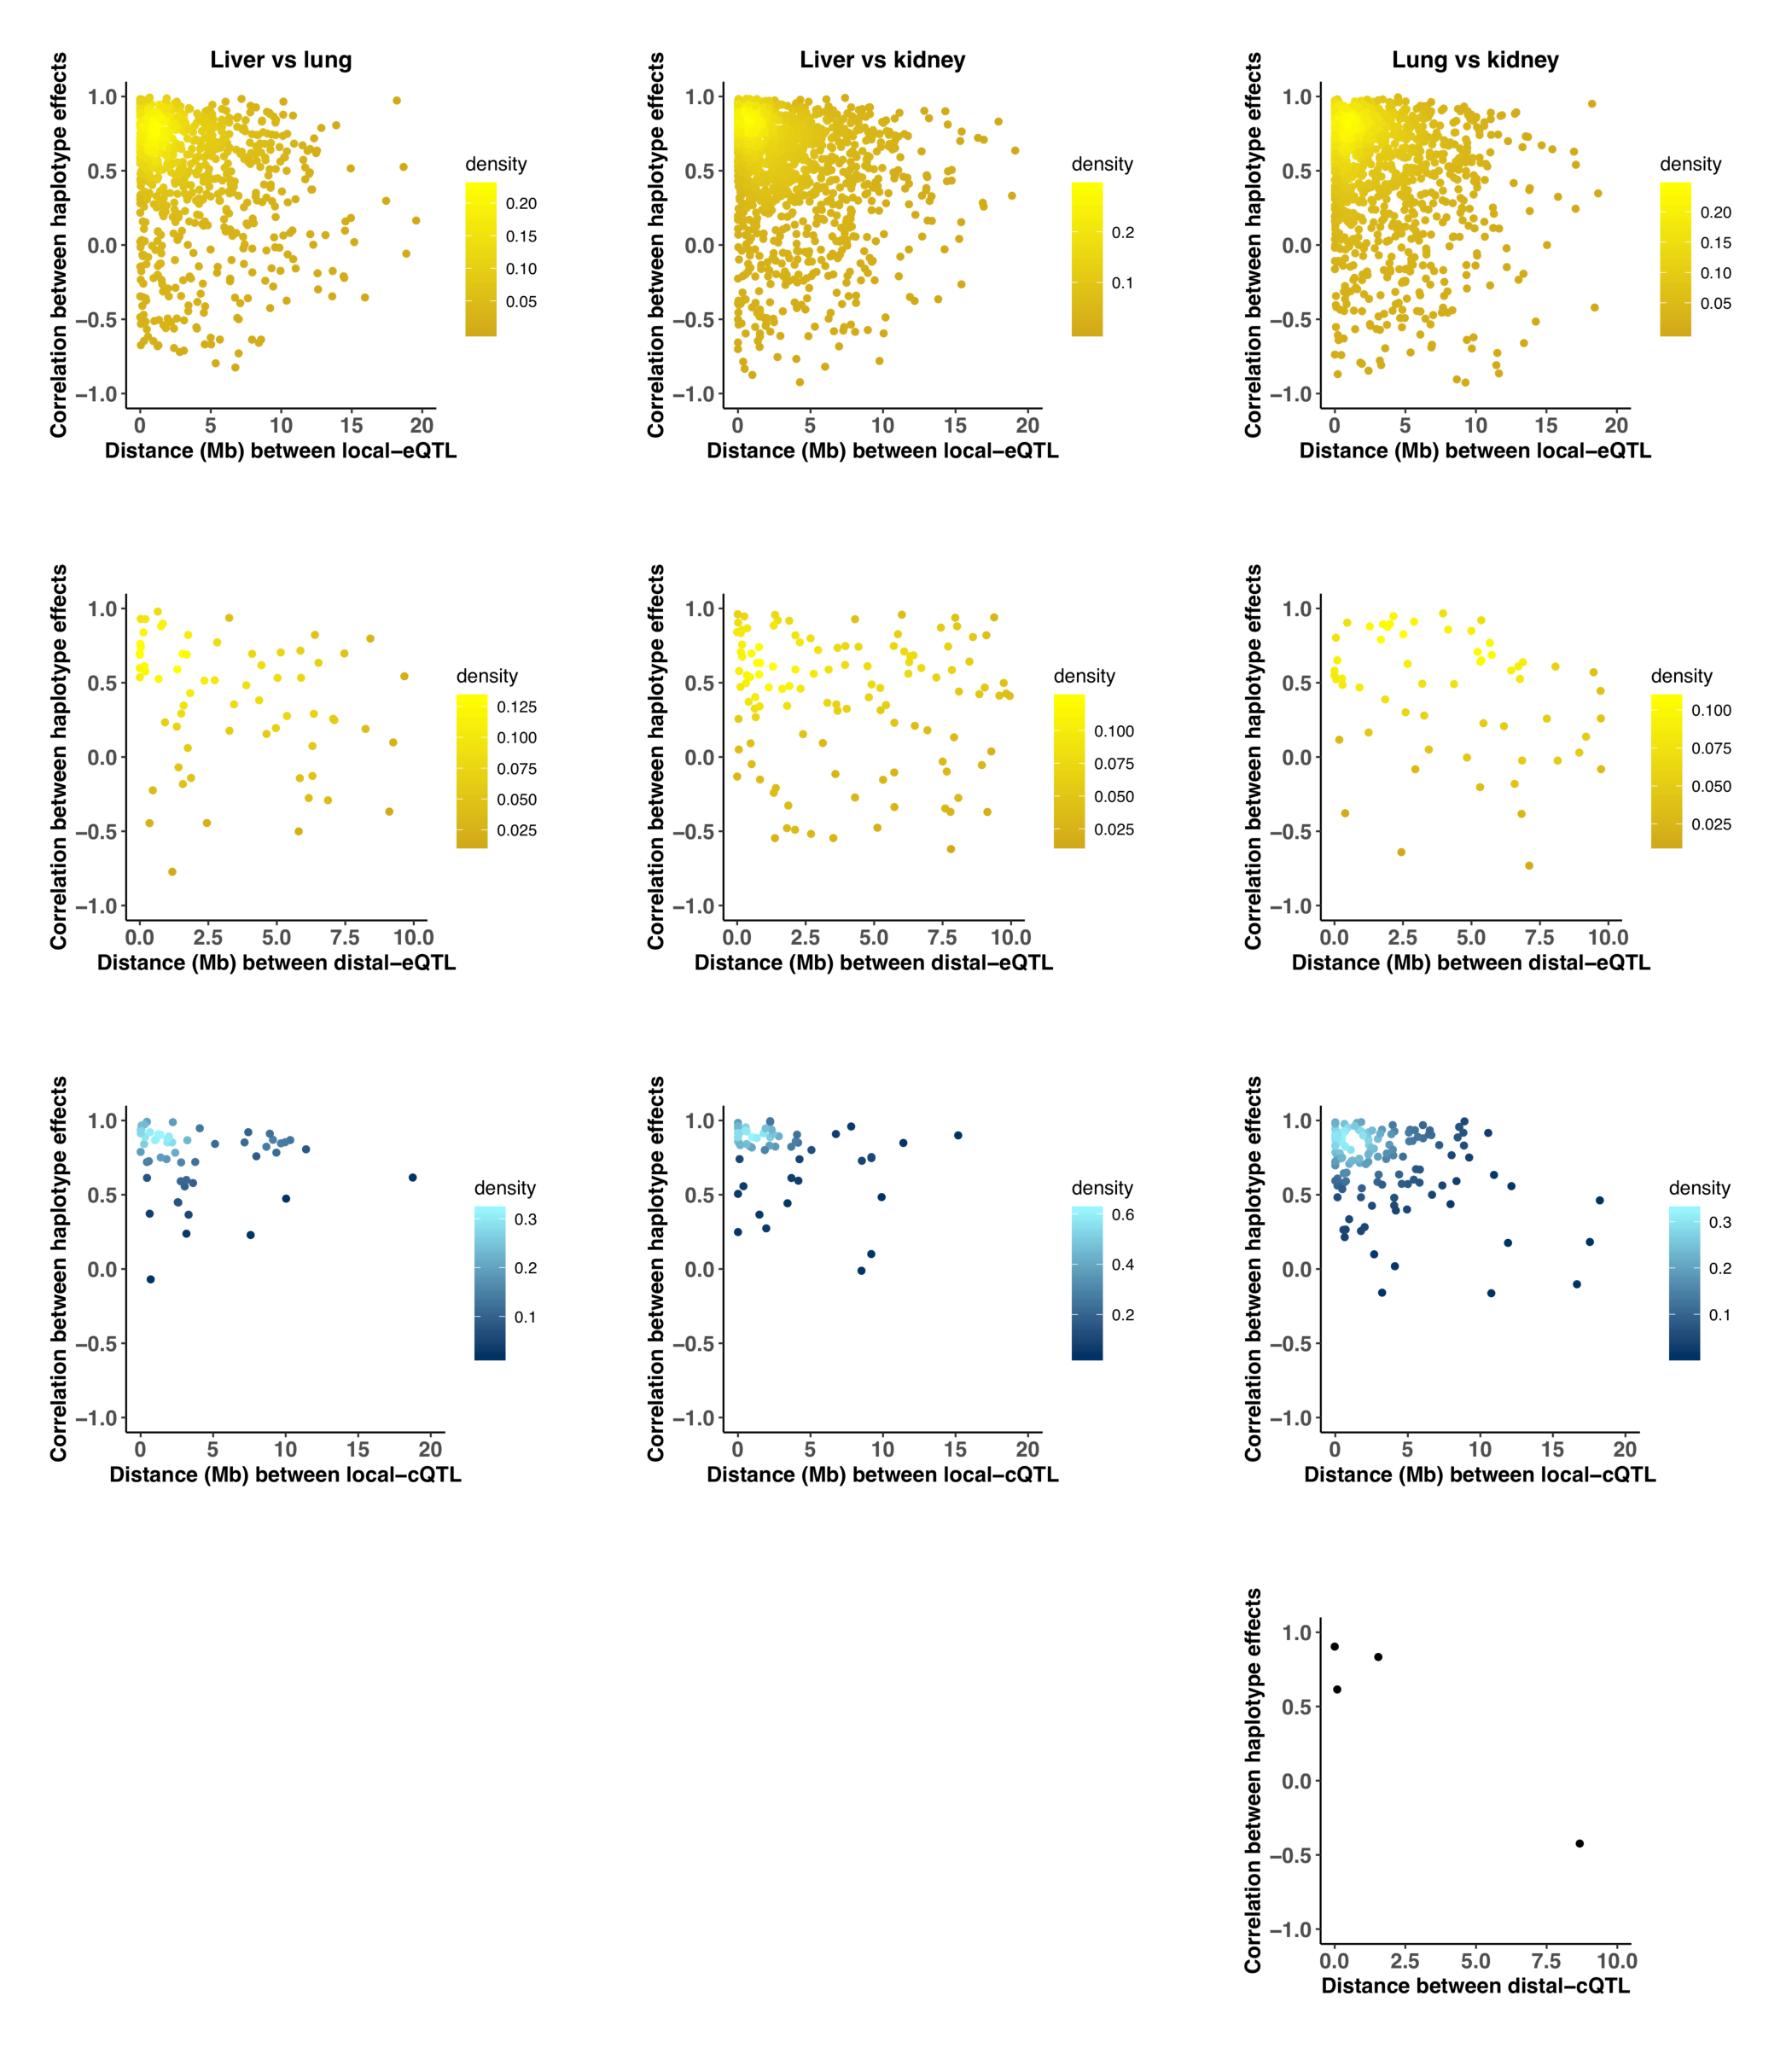
\includegraphics[width=0.9\textwidth, trim={0in 0in 0in 0in}, clip]{figs/effect_size_cor_by_dist.pdf}
\caption{\textbf{QTL pairs with highly correlated founder allele effects map proximally to each other.} Founder effects were estimated as constrain BLUPs. Pairwise correlations of the 8-element effect vectors were calculated for QTL pairs, and plotted again the distance between the QTL coordinates in Mb for (liver/lung) in the left column, (liver/kidney) in the middle column, and (lung/kidney) in the right column. Single eQTL and cQTL pairs are represented as a yellow and blue dots, respectively. Local-eQTL are shown in the top row, distal-eQTL in the second row, local-cQTL in the third row, and distal c-QTL in the bottom row, for which only four pairs were detected in (lung/kidney).
\label{fig:qtl_cor_by_distance_comparison}}
\end{figure*}

\begin{figure*}[hp]
\renewcommand{\familydefault}{\sfdefault}\normalfont
\centering
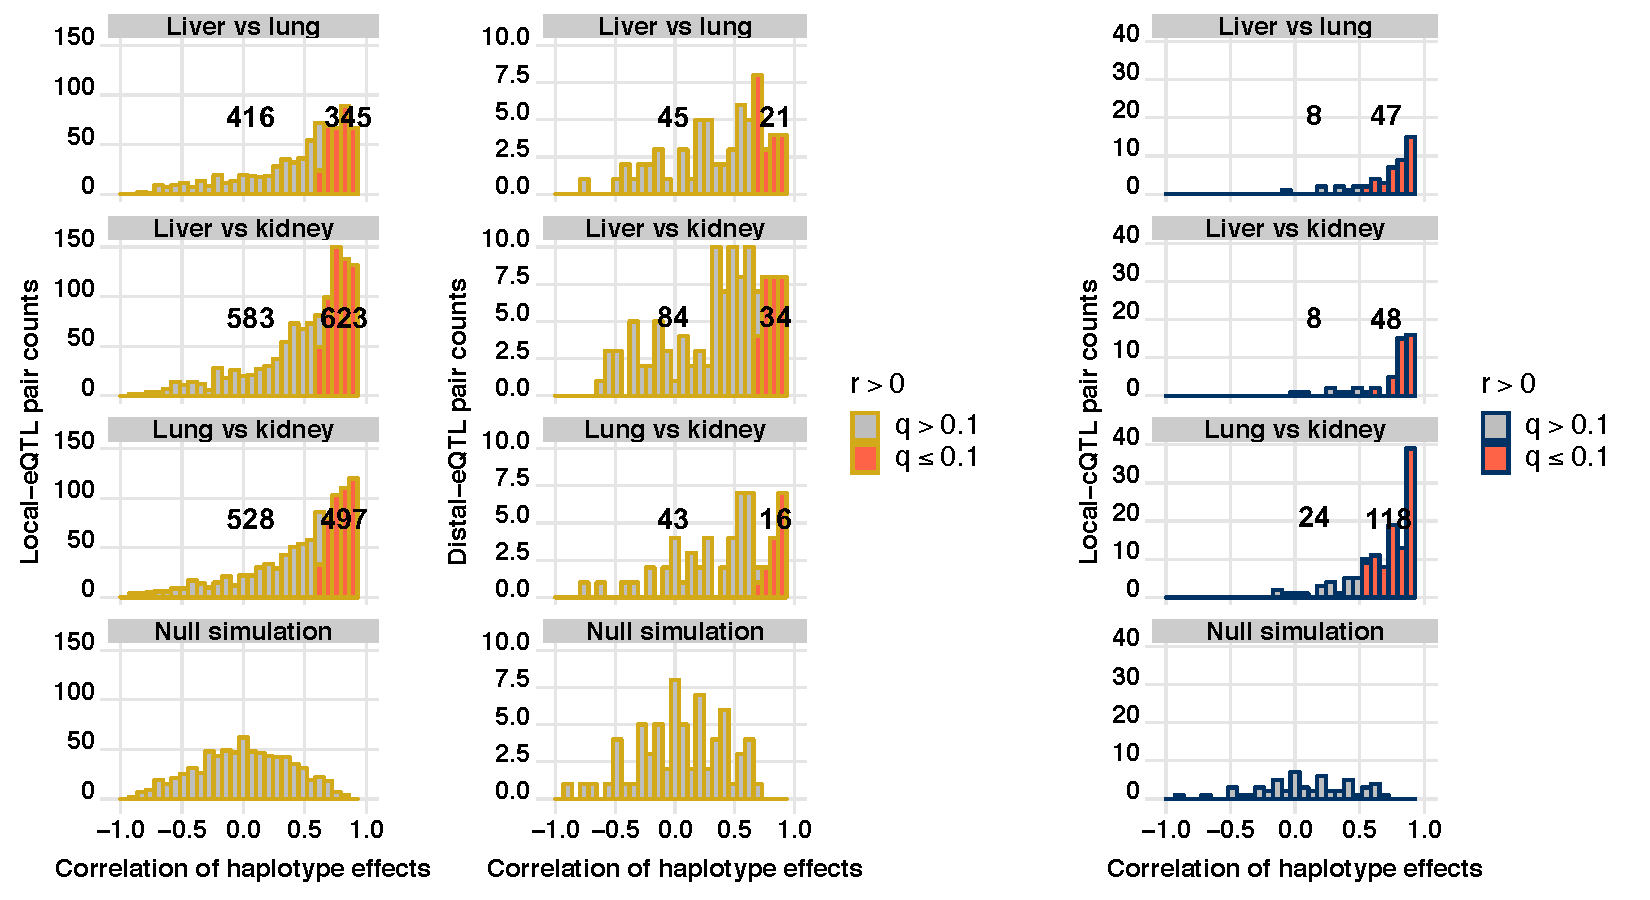
\includegraphics[width=\textwidth, trim={0in 0in 0in 0in}, clip]{figs/qtl_pair_cor_histograms.pdf}
\caption{\textbf{Consistent genetic regulation of gene expression and chromatin accessibility observed across tissues.} Enrichment of significantly correlated founder allele effects detected in QTL pairs for gene expression and chromatin accessibility. Pairs of QTL observed in multiple tissues were defined for local-eQTL (left column), distal-eQTL (middle column), and local-cQTL (right column). Only four pairs of distal-cQTL were observed, all shared between lung and kidney. A right-tailed test the correlation between founders effects ($H_{A}: r > 0$) was performed for each QTL pair, producing p-values that were then FDR adjusted. Null simulations of uncorrelated 8-element vector pairs for each class of QTL and pairwise tissue comparison emphasize the observed enrichment in correlated founder effects between QTL pairs.  
\label{fig:qtl_pair_histograms}}
\end{figure*}

\begin{figure*}[hp]
\renewcommand{\familydefault}{\sfdefault}\normalfont
\centering
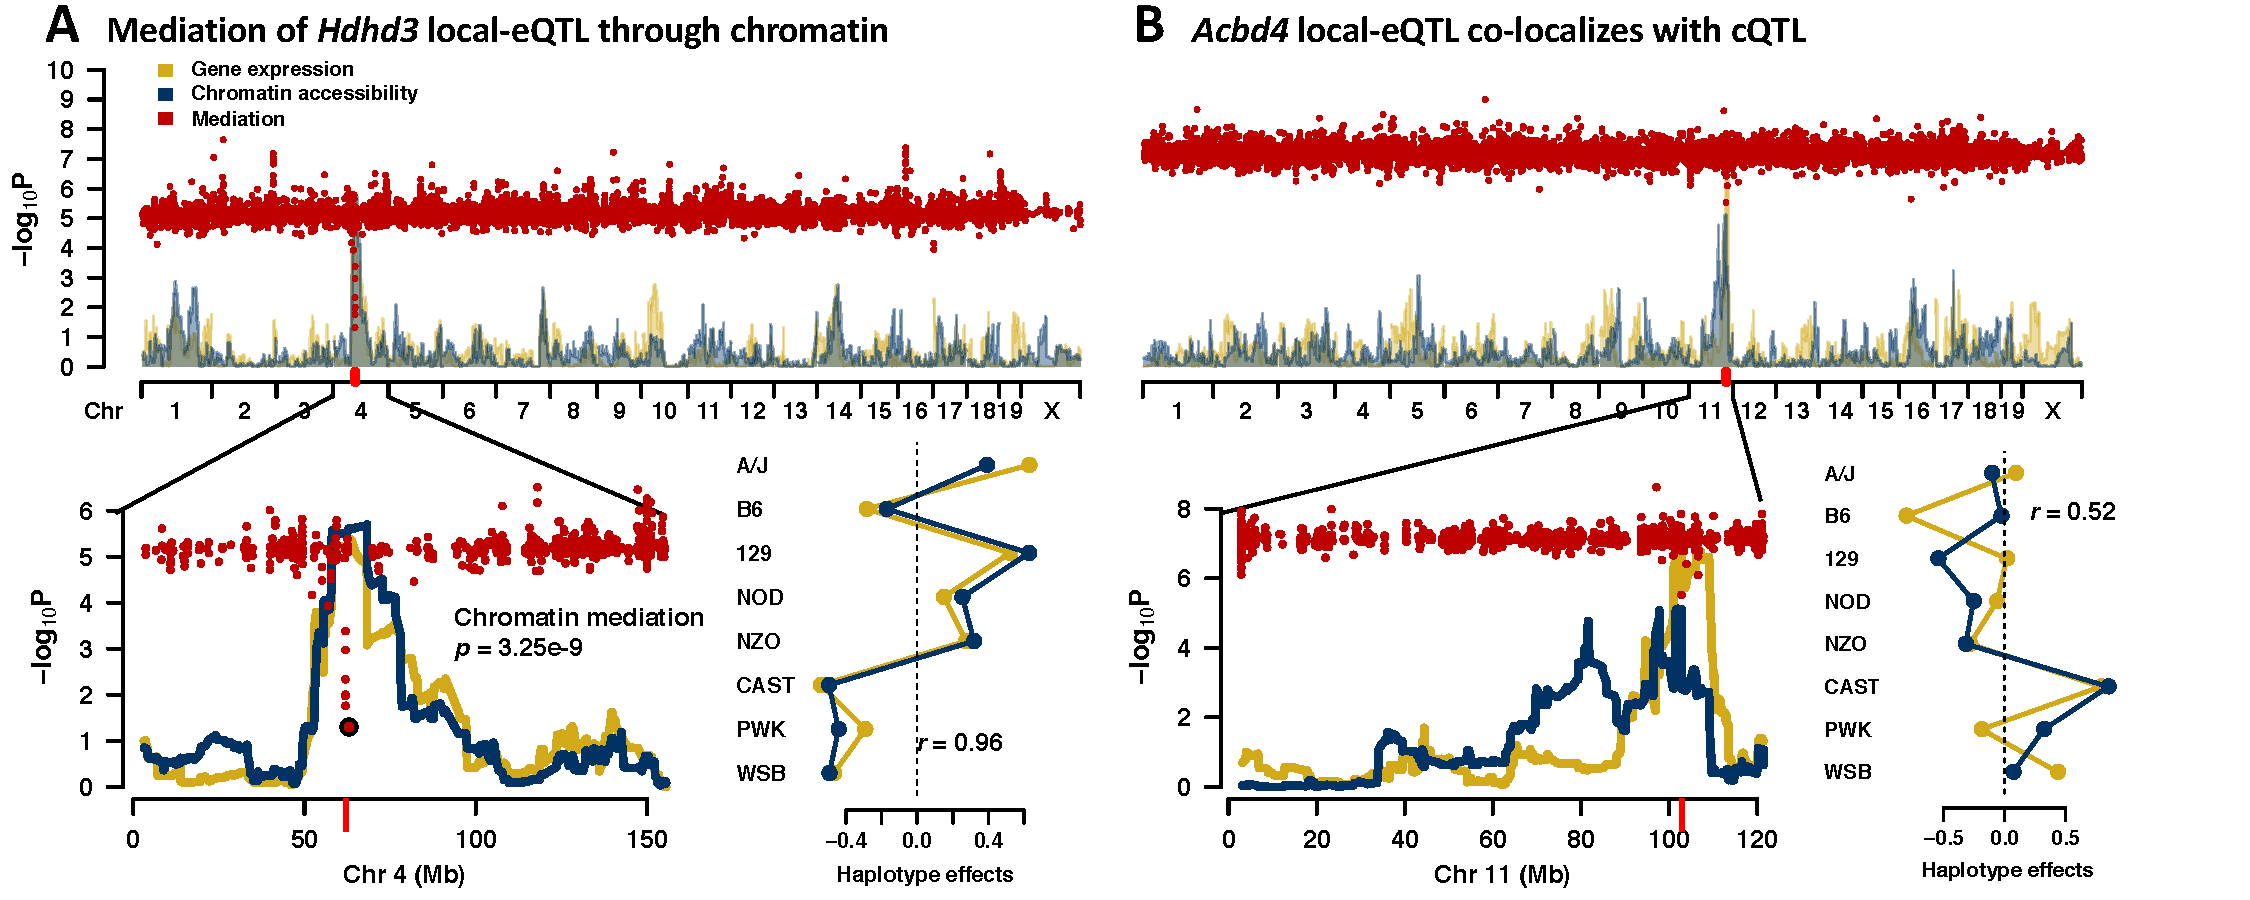
\includegraphics[width=\textwidth]{figs/mediation_or_colocal.pdf}
\caption{\textbf{Co-localizing eQTL and cQTL are not sufficient for statistical mediation.} The approach used to detect mediation through chromatin accessibility requires that the eQTL and cQTL co-localize (both within 10 Mb of the gene TSS), as well as possess similar founder allele effect patterns. Co-localizing cQTL are observed for local-eQTL for both \textit{Hdhd3} in liver \textbf{[left]} and \textit{Acbd4} in kidney \textbf{[right]}. QTL and mediation scans are included (\textbf{[top]}), with chromosomes 4 and 11 blown up for \textit{Hdhd3} and \textit{Acbd4}, respectively. The red ticks denote the TSS for both genes. The founders effects were estimated as centered and scaled BLUPs. The founder effects for the eQTL and cQTL are highly correlated ($r = 0.96$) for \textit{Hdhd3}, but not for \textit{Acbd4} ($r = 0.52$). Strong mediation of the \textit{Hdhd3} eQTL through chromatin is detected, but not for \textit{Acbd4}. The effect size of the proximal cQTL to \textit{Acbd4} is smaller than its eQTL, also inconsistent with the relationship depicted in \textbf{Figure \ref{fig:graph}[top]}.\label{fig:colocalization}}
\end{figure*}

\begin{figure*}[hp]
\renewcommand{\familydefault}{\sfdefault}\normalfont
\centering
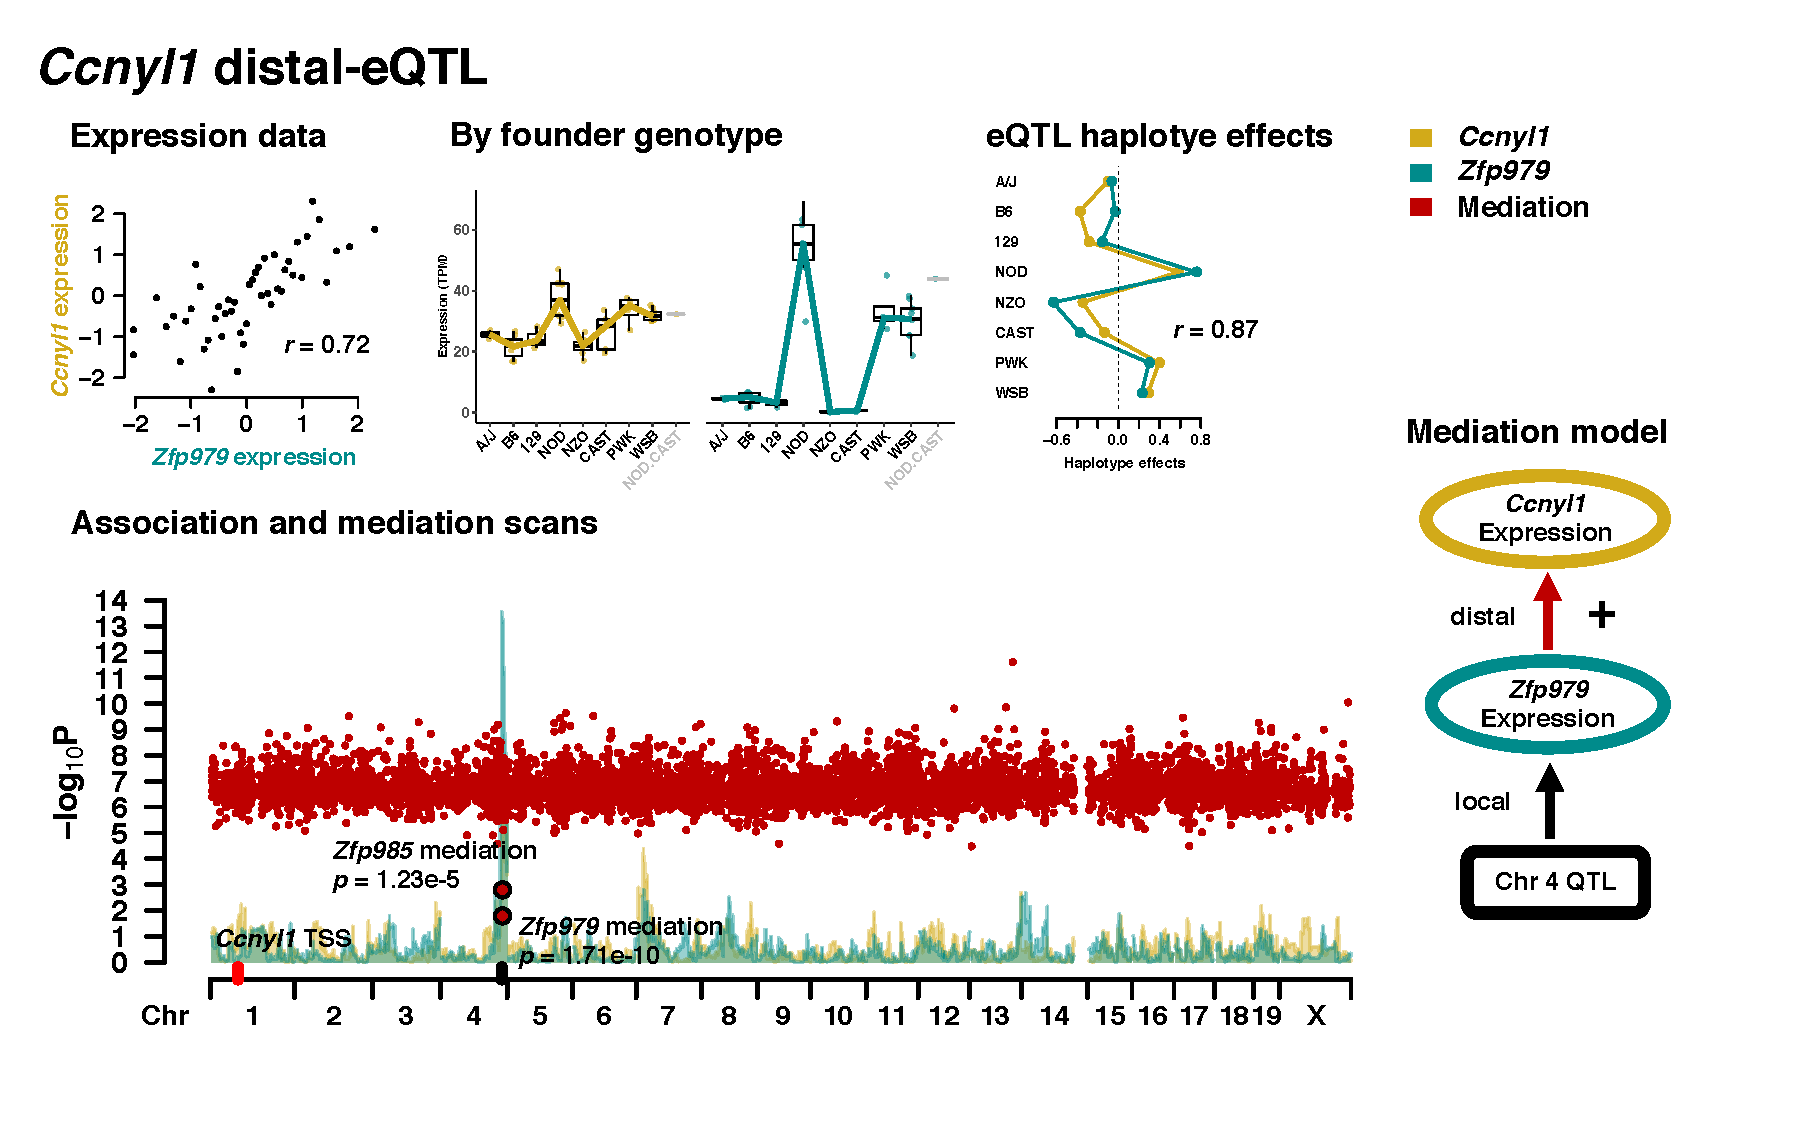
\includegraphics[width=\textwidth, trim={0in 0.5in 0in 0in}, clip]{figs/ccnyl1_mediation.pdf}
\caption{\textbf{Mediation of \textit{Ccnyl1} distal-eQTL through \textit{Zfp979} expression.} Expression of \textit{Ccnyl1} and \textit{Zfp979} are correlated ($r = 0.72$) in lung, which is also observed in the expression data categorized by diplotype and the founder effects estimated as scaled BLUPs. The distal-eQTL on chromosome 4 for \textit{Ccnyl1} corresponds closely to local-eQTL of \textit{Zfp979}. \textit{Ccnyl1} is located on chromosome 1, indicated by the red tick. \textit{Zfp979} and \textit{Zfp985}, both zinc finger proteins likely with DNA binding properties, are identified as strong candidate mediators of the distal-eQTL at genome-wide significance. The correlations, magnitude of effects, and mediation are consistent with the simple relationship depicted in the graph on the \textbf{[right]}. The distal-eQTL and candidate mediators are located in the same region of interest defined in \cite{HamiltonWilliams2013}, which also regulates \textit{Akr1e1} expression. 
\label{fig:ccnyl1_exmediation}}
\end{figure*}

\begin{figure*}[hp]
\renewcommand{\familydefault}{\sfdefault}\normalfont
\centering
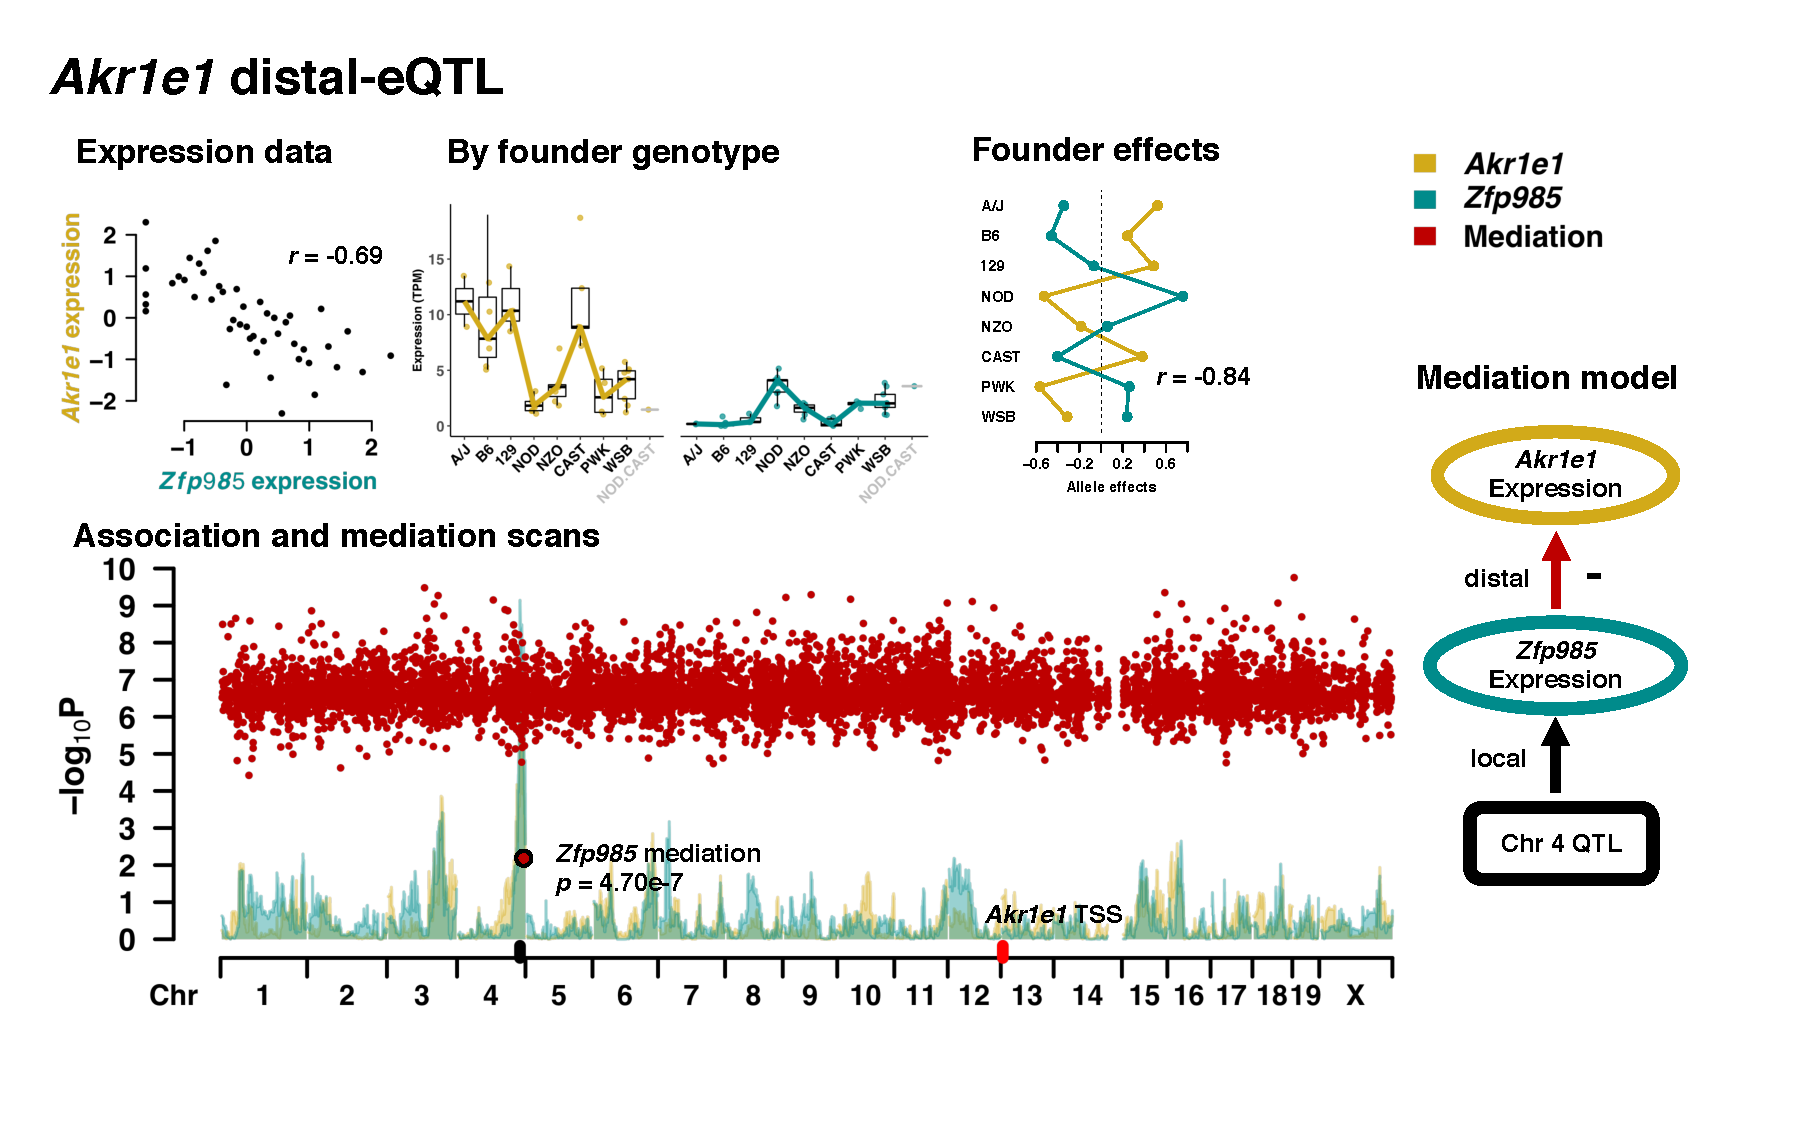
\includegraphics[width=\textwidth, trim={0in 0.5in 0in 0in}, clip]{figs/akr1e1_mediation.pdf}
\caption{\textbf{Mediation of \textit{Akr1e1} distal-eQTL through \textit{Zfp985} expression.} Expression of \textit{Akr1e1} and \textit{Zfp985} are anti-correlated ($r = -0.69$) in lung. This relationship is also observed in the expression data plotted as boxplots, categorized by most likely diplotype, and the founder allele effects, estimated as scaled BLUPs. The QTL and mediation scans reveal that \textit{Akr1e1}, TSS marked with a red tick on chromosome 13, possesses a distal-eQTL on chromosome 4 that is proximal to the strong local-eQTL of \textit{Zfp985}. The mediation scan identifies \textit{Zfp985} as a strong candidate mediator consistent with the mediation model included on the \textbf{[right]}. A more complete picture of the genetic regulation of \textit{Akr1e1} expression is pieced together by looking across all three tissues and includes a potential chromatin mediator (\textbf{Figure \ref{fig:akr1e1_full_model.pdf}}).
\label{fig:akr1e1_exmediation}}
\end{figure*}

\begin{figure*}[hp]
\renewcommand{\familydefault}{\sfdefault}\normalfont
\centering
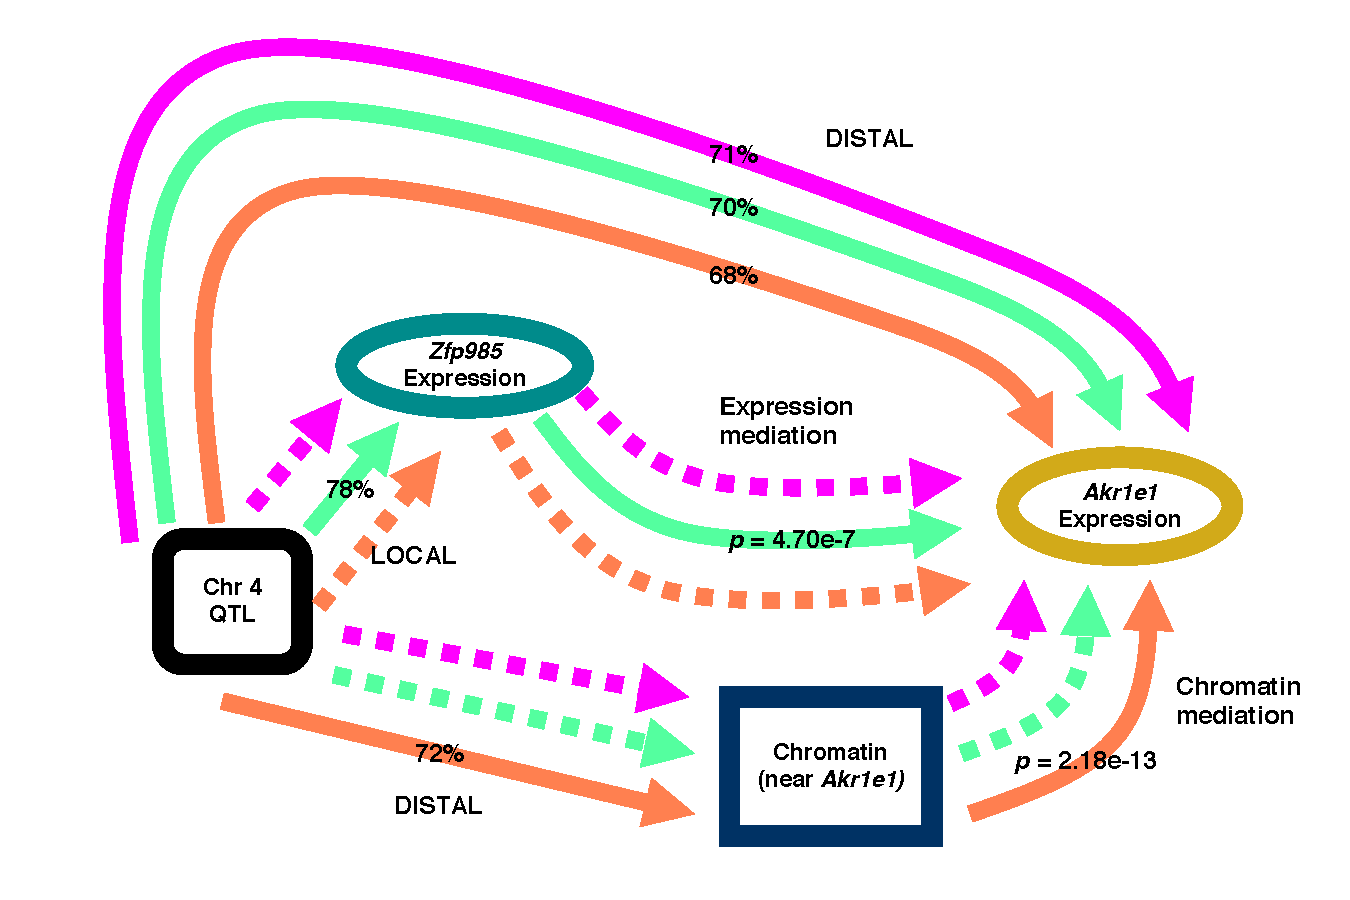
\includegraphics[width=\textwidth, trim={0in 0in 0in 0in}, clip]{figs/akr1e1_observed_relationships.pdf}
\caption{\textbf{Observed relationships across the three tissues related to the genetic regulation of \textit{Akr1e1} expression.} The model for the distal genetic regulation of \textit{Akr1e1} expression, described in \textbf{Figure \ref{fig:akr1e1_full_model}}, was reconstructed from these observed relationships. Solid arrows were observed, whereas dashed arrows are assumed. QTL effect sizes were estimated using Eq \ref{eq:effect_size}, and mediation p-values (permP) were defined using a permutation procedure. The assumed relationships are supported by the presence of the distal-eQTL in all three tissues.
\label{fig:akr1e1_relationships}}
\end{figure*}


